\documentclass[12pt, a4paper]{extarticle}

\usepackage{polyglossia}
\setmainlanguage{english} % Язык по-умолчанию русский с поддержкой приятных команд пакета babel
\setotherlanguage{russian} % Дополнительный язык = английский (в американской вариации по-умолчанию)
\newfontfamily\cyrillicfonttt{Fira Mono for Powerline}[Scale=MatchLowercase] % моноширинный шрифт для кириллицы
\defaultfontfeatures{Ligatures=TeX} % стандартные лигатуры TeX, замены нескольких дефисов на тире и т. п. Настройки моноширинного шрифта должны идти до этой строки, чтобы при врезках кода программ в коде не применялись лигатуры и замены дефисов
\setmainfont{CMU Serif} % Шрифт с засечками
\setsansfont{CMU Sans Serif} % Шрифт без засечек
\setmonofont{Fira Mono for Powerline} % моноширинный шрифт

\usepackage[backend=biber, style=numeric-comp, language=auto, autolang=other, sorting=none]{biblatex}
\addbibresource{references.bib}

\usepackage[cache=false]{minted}
\usepackage{amsmath}
\usepackage{unicode-math}
\usepackage{float}
\usepackage{caption, subcaption}
\usepackage{geometry}
\usepackage{graphicx}
\usepackage{titlesec}
\usepackage{enumitem}
\usepackage{indentfirst}
\usepackage{listings}
\usepackage{xcolor}
\usepackage{longtable}
\usepackage{xltabular}
\usepackage{appendix}
\graphicspath{{./images/}}
\geometry{left=30mm,
          right=10mm,
          top=20mm,
          bottom=20mm}

\usepackage{colortbl}
\usepackage{hhline}
\usepackage{xcolor}

\usepackage{wrapfig}
\usepackage{microtype}
\usepackage{tabularx}

\usepackage{array}
\usepackage{multirow}

%\pretolerance=5000
%\tolerance=9000
%\hyphenpenalty=1000
%\emergencystretch=0pt

\usepackage{booktabs}
\usepackage[colorlinks=true,linkcolor=black,urlcolor=black,citecolor=black]{hyperref}

\lstdefinestyle{bash}{
    basicstyle=\ttfamily,
    framerule=10pt,
    breakatwhitespace=false,
    breaklines=true,
    captionpos=b,
    keepspaces=true,
    showspaces=false,
    showstringspaces=false,
    showtabs=false,
    tabsize=2,
    columns=fullflexible,
    literate={-}{-}1
}

\lstset{style=bash}
\setmathfont{Latin Modern Math}

%\setlist[itemize]{noitemsep}
%\setlist[enumerate]{noitemsep}

\renewcommand{\baselinestretch}{1.5}

\date{\today}

\begin{document}

\begin{titlepage}
{\small
    \begin{center}
         NATIONAL RESEARCH UNIVERSITY HIGHER SCHOOL OF ECONOMICS
        \\
        \textit{Tikhonov Moscow Institute of Electronics and Mathematics}
   \end{center}

	\vfill

	\begin{center}
		\textbf{
            Resiliently Synchronizing SFN Networks: \\Combining Precise Time Signals from GPS and Longwave Radio Stations
        }

        \vspace{1em}

        by \\
        Maxim Emelyanenko
	\end{center}

    \vspace{1.5em}

	\begin{center}
        Graduate Qualification Work -- Bachelor Thesis\\
        Bachelor of Science in Information Security (10.03.01)
	\end{center}

	\vfill

    \begin{tabbing}
    \hspace{1.35in} \= \hspace{1in} \kill

    Authored by: \> Maxim Emelyanenko \\
                 \> Department of Information Security \\
                 \> Group BIB201 \\

    \vspace{2em} \\

    Certified by: \> Yaroslav Mesheryakov \\
                  \> Associate Professor, Thesis Supervisor \\
    \end{tabbing}

	\begin{center}
		Moscow 2024
	\end{center}
}

\end{titlepage}

\addtocounter{page}{1}

\tableofcontents
\pagebreak

\section*{Annotation}
\addcontentsline{toc}{section}{Annotation}
This thesis introduces a novel hybrid approach to enhance the resilience of
time synchronization within Single Frequency Networks (SFN), crucial for
digital broadcasting systems. The traditional reliance on Global Navigation
Satellite Systems (GNSS) exposes SFNs to vulnerabilities including geophysical
phenomena like ionospheric variations due to solar activity fluctuations, and
deliberate disruptions such as spoofing and jamming attacks.

To address these vulnerabilities, this work integrates terrestrial longwave
radio transmitters into the time transfer framework as a supplementary
precise time signal source. By leveraging the stable and reliable nature of
longwave signals, a dual-check mechanism is implemented, enhancing the SFN's
reliability significantly. This integrated system provides a robust fallback,
ensuring continuous operation even when GNSS services are compromised.

Experimental validations confirm the effectiveness of this approach,
demonstrating a reduction in time transmission errors and an enhanced resilience
against spoofing and jamming within SFNs.

The findings lay a foundation for future research and development in robust
hybrid time synchronization technologies, offering a scalable and effective
solution to safeguard critical infrastructure against single-source dependency
risks.

\section*{Аннотация}

\begin{otherlanguage}{russian}
    В работе представлен новый метод синхронизации времени в одночастотных
    сетях (SFN) для повышения устойчивости систем цифрового вещания. Описанный
    метод устраняет критические уязвимости, присущие традиционно используемым
    для синхронизации времени глобальным навигационным спутниковым системам
    (GNSS). К числу факторов, к которым уязвимы сети SFN, работающие на основе
    сигналов GNSS, относятся как геофизические явления, например, ионосферные
    изменения в результате перепадов солнечной активности, так и преднамеренные
    воздействия.

    Решение описанной проблемы осущствлено путем интеграции в службу точного
    времени наземных длинноволновых радиопередатчиков в качестве
    дополнительного источника сигналов точного времени. В работе предложена
    более устойчивая, по сравнению с имеющейся, структура передачи параметров
    точного времени. Для этого использована двухуровневая проверка, значительно
    повышающая надежность работы SFN. Такая интеграция наземных длинноволновых
    радиопередатчиков в службу точного времени использует стабильный и надежный
    характер длинноволновых сигналов для создания отказоустойчивого механизма,
    обеспечивающего непрерывную работу в условиях потенциальных отказов работы
    GNSS.

    Экспериментальная проверка подтвердила эффективность этого метода: в
    результате его применения снизилось количество ошибок передачи времени и
    усилилась защита сети SFN от спуфинга и атак глушения.

    Результаты создают основу для будущих исследований и разработок в области
    надежной гибридной системы синхронизации точного времени. Предложено
    масштабируемое и эффективное решение для защиты критически важных
    инфраструктур против внешних факторов.
\end{otherlanguage}

\vfill

\textbf{Keywords:}
Time Transfer, Time Cross-checking, GNSS, SFN, Spoofing

\pagebreak

\section{Introduction}

%With single frequency networks evolving to meet ever-increasing throughput
%demands,  the precision of timing synchronization becomes crucial for the
%network performance. The advent of Digital Video Broadcasting -- Terrestrial
%(DVB-T) standard and their subsequent enhancements in DVB-T2 have significantly
%raised the bar for synchronization accuracy. These standards, employing
%orthogonal frequency-division multiplexing (OFDM) modulation, offer substantial
%data throughput but also introduce strict requirements for transmission
%synchronization to prevent inter-symbol interference and optimize bandwidth
%utilization~\cite{ETSIDVBT22009,liang2007timing}. Historically, GNSSs, such as
%GPS and GLONASS, have been the cornerstone for achieving this level of
%synchronization across the geographically distributed infrastructure of SFNs
%because other systems like Precision Time Protocol (PTP), while effective in
%certain contexts with consistent network latencies, like a localized data
%center, encounter scaling challenges over geographical expanses, rendering them
%unsuitable~\cite{ieee1588_2008,ptpscale}. However, the reliance on GNSS without
%any complementary or backup system introduces a range of vulnerabilities,
%including susceptibility to ephemeris errors, ionospheric delays, solar
%activities, and potential security threats like jamming and spoofing, which are
%thoroughly assessed in the Section~\ref{gnss-vuln}. These vulnerabilities not
%only compromise the integrity and reliability of broadcast services but also
%highlight a critical single point of failure within the time transfer
%framework of SFNs.
%
%To mitigate similar risks in the context of global navigation, the eLoran
%system was developed as a terrestrial-based alternative to GNSS, designed to
%offer a robust solution to the single point of failure issue by providing a
%complementary source of timing signals usable for positional trilateration~\cite{eloran}.
%The approaches suggested by eLoran are further reviewed in this paper in the
%section~\ref{eloran-chap}.
%
%Inspired by the principles of eLoran, this study explores the feasibility of
%leveraging terrestrial radio stations, specifically those managed by the
%Russian State Service for Time, Frequency, and Earth Rotation Parameters,
%alongside similar stations in Germany, the United Kingdom, and Japan~\cite{itur1997standard}.
%These stations, characterized by their picosecond-precision in time signal
%dissemination, present a viable solution for enhancing SFN synchronization
%resilience and accuracy~\cite{vniiftri}.

%%%

The rapid evolution of single frequency networks (SFNs) necessitates heightened
precision in timing synchronization to accommodate the increasing data
throughput demands. This is particularly critical with the advent of advanced
broadcasting standards such as Digital Video Broadcasting -- Terrestrial
(DVB-T) and its enhancement in DVB-T2. While the focus is on DVB-T2 due to its
extensive use in Russia~\cite{fcp}, the findings and methodologies proposed by
this paper are applicable to other digital broadcasting standards such as ATSC,
ISDB-T, and DTMB, which are used in different regions around the world. These
standards generally utilize an orthogonal frequency-division multiplexing (OFDM)
modulation, which imposes stringent synchronization requirements to prevent
inter-symbol interference and maximize bandwidth
efficiency~\cite{ETSIDVBT22009,liang2007timing,morshed2009synchronization,ofdm}.

Historically, Global Navigation Satellite Systems (GNSS) such as GPS and
GLONASS have been instrumental in achieving high precision time synchronization
across the extensive and geographically dispersed infrastructure of SFNs.
However, GNSS systems have numerous vulnerabilities, including susceptibility
to ephemeris errors, ionospheric delays, solar activities, and security threats
like jamming and spoofing. These vulnerabilities are detailed in
Section~\ref{gnss-vuln}, highlighting the critical need for alternative or
complementary systems to enhance reliability and integrity in SFN
synchronization.

An alternative approach, inspired by the eLoran system, is explored in this
study. eLoran is a terrestrial-based navigation system developed to provide a
reliable backup for GNSS, ensuring resilience against a single point of failure
in critical synchronization applications~\cite{eloran}. Further discussions on
eLoran's applicability and implementation are presented in
Section~\ref{eloran-chap}.

Building upon the eLoran principles, this thesis examines the feasibility of
utilizing terrestrial radio stations, specifically those managed by the Russian
State Service for Time, Frequency, and Earth Rotation Parameters, alongside
stations in Germany, the United Kingdom, and Japan.
These stations are renowned for their picosecond-level precision in time signal
broadcasting and represent a promising alternative for enhancing
synchronization accuracy and resilience in SFNs~\cite{itur1997standard}.


\subsection{Objective}

This thesis aims to develop and validate resilient time transfer methodologies
that enhance the resilience of synchronization in Single Frequency Networks
(SFN), crucial for reliable digital broadcasting. Given the inherent
vulnerabilities of Global Navigation Satellite Systems (GNSS) such as GPS and
GLONASS --- ranging from ionospheric variations to intentional disruptions like
spoofing and jamming --- this work proposes the integration of terrestrial
longwave radio signals as a supplementary precision time source. This hybrid
synchronization approach seeks to mitigate the risks associated with GNSS
dependencies by ensuring a continuous operation through alternative time signals,
thereby fostering enhanced resilience and reliability of SFN infrastructures
worldwide. The ultimate goal is to demonstrate that the integration of these
terrestrial signals can significantly reduce synchronization errors and
safeguard against the potential failure of GNSS, thus providing a more stable
and secure broadcasting environment.

This paper is organized in the following way: Section~\ref{sec:theory} provides
a theoretical background on the working principles and vulnerabilities of GNSS
and the synchronization requirements of SFNs, Section~\ref{sec:methods} details
the methods employed in the experimental evaluation,
Section~\ref{sec:time-transfer} discusses the integration and testing of time
transfer techniques, and Section~\ref{sec:resilient-time-transfer} explores
resiliency improvements to the time transfer techniques against GNSS jamming
and spoofing scenarios. Finally, Section~\ref{sec:concl} concludes with a
summary of the findings and implications for future research.

\subsection{Theoretical Background}\label{sec:theory}

\subsubsection{Time Transfer Approaches}

Time synchronization in Single Frequency Networks (SFNs) can be primarily
categorized into the one-way and two-way synchronization techniques, each having
its unique application and accuracy profile suitable for different levels of
system demands.

\textbf{One-Way Time Transfer:} In the one-way time transfer, a time signal is sent
from a source to a receiver without requiring any information to be sent back
to the source. This method is simpler and often used where high precision is
not paramount. However, its accuracy can be affected by asymmetries in signal
path delays, which are not typically compensated for in the one-way method.
This approach is often employed in systems where the absolute precision of
synchronization is less critical but where the simplicity and
cost-effectiveness of the setup are prioritized.

\textbf{Two-Way Time Transfer:} Two-way time transfer involves sending a time
signal from a source to a receiver, which then sends a return signal back to
the source. The time of flight for the signals is measured and used to adjust
and correct any delay, thus providing a higher level of accuracy compared to
the one-way transfer. This method compensates for path delay variations and is
crucial in applications requiring high precision, such as in telecommunications
and high-frequency trading systems~\cite{two-way-time-transfer}.

\textbf{Stratum Levels in Network Synchronization:} In network time
synchronization, stratum levels define the hierarchy of sources providing the
timing. A stratum 1 time server is directly connected to a primary time source,
such as a GPS or a radio clock. Lower stratum numbers represent closer
proximity to the primary time standard, and thus generally higher accuracy.
Devices downstream, such as stratum 2 servers, synchronize to stratum 1
servers, adding a degree of latency and potential error as the stratum number
increases. This hierarchical setup ensures that even if lower stratum devices
have less precision, the system as a whole can maintain a robust and scalable
time synchronization infrastructure.

\subsubsection{Working Principle of GNSS}

Global Navigation Satellite Systems (GNSS) operate on the principle of
trilateration, utilizing signals from multiple satellites to pinpoint a
receiver's location. Each satellite transmits messages that include the
satellite's position and the time the message was sent. Receivers calculate the
distance to each satellite by measuring the time delay of the received signals,
which, when combined with the positions of at least four satellites, allow for
accurate determination of the receiver's three-dimensional position and time.

GNSS signals are encoded using a technique known as spread spectrum. Each
satellite broadcasts a unique pseudorandom noise (PRN) code, which helps to
distinguish between signals from different satellites and assists in precise
timing measurements necessary for trilateration.

\textbf{Real-Time Kinematic (RTK):} RTK is a technique used to enhance the
precision of position data derived from satellite-based positioning systems. It
uses measurements of the phase of the satellite's signal carrier wave in
addition to the information content of the signal and relies on a single
reference station to provide real-time corrections, achieving precision down to
centimeters~\cite{high-precision-rtk, patent}.

\textbf{Differential Carrier Phase Time Transfer:} This method utilizes the
carrier phase of GNSS signals for high-precision time transfer. By comparing
the phase difference of the carrier signals received from a satellite at two or
more locations (typically a reference station and a remote station), the
relative timing errors can be minimized significantly. This technique is
especially useful in applications requiring extremely high accuracy and
stability in time synchronization~\cite{carrier-phase-measurement}.

\subsubsection{GNSS Vulnerabilities}\label{gnss-vuln}

Global Navigation Satellite Systems (GNSS) face a spectrum of vulnerabilities
that impact the accuracy and reliability of synchronization in Single Frequency
Networks (SFN). Technical errors such as ephemeris inaccuracies and time system
errors can lead to significant deviations in positioning and timing
signals~\cite{dempster2001vulnerable}. Additionally, natural phenomena like
ionospheric and tropospheric delays, compounded by solar activities, cause
signal distortion and interference~\cite{infrastructure2001vulnerability}.

Beyond natural and technical issues, intentional interferences such as jamming
and spoofing present severe threats. Jamming disrupts GNSS reception, while
spoofing misleads receivers with counterfeit signals. Notably, incidents in
South Korea due to GPS jamming by North Korea exemplify the growing risk and
sophistication of these attacks~\cite{SeoKim2013}. The intrinsic low power of
GNSS signals heightens their susceptibility to such disruptions~\cite{time-sync-attacks}.

The dependency of SFNs on accurate time synchronization makes them particularly
prone to the adverse effects of GNSS vulnerabilities. These issues underline
the urgent need for developing and integrating alternative synchronization
methods to ensure the security and reliability of critical infrastructures
like digital broadcasting services. The exploration of robust countermeasures
is crucial to mitigate the impact of GNSS vulnerabilities on SFN operations, as
emphasized by recent studies on the consequences of GNSS
disruptions~\cite{machaj2021impact}.

\subsubsection{SFN Synchronization}\label{sfn-sync}

Single Frequency Networks (SFNs) necessitate precise synchronization of
broadcast signals across multiple transmitters to ensure seamless delivery and
prevent signal interference, crucial for maintaining high network efficiency
and signal quality. Traditionally, SFNs have relied on GNSS systems like GPS
and GLONASS for synchronization. Although effective, this method introduces
vulnerability due to its single point of failure nature, highlighting the need for
more resilient synchronization techniques.

An alternative, the Integrated Time Transfer via the Nimbra transport platform,
embeds time signals within the data stream transmitted across physical networks. Each
node in the network utilizes these embedded signals to synchronize its
operations. While this method enhances resilience against GNSS vulnerabilities
such as jamming and spoofing, it depends heavily on the network
infrastructure's integrity, which can be compromised by high latency or
inconsistent network designs~\cite{Hellstrom2007,ptpscale}.

The shift towards such alternative synchronization methods introduces
significant technical and infrastructural challenges. Establishing a
terrestrial time signal network, for instance, demands considerable investment
and meticulous planning to achieve the necessary coverage, precision, and
reliability. Moreover, integrating multiple synchronization sources adds
complexity to synchronization algorithms and system designs, necessitating
ongoing research and development to ensure effective implementation across
diverse network configurations.

\subsubsection{eLoran}\label{eloran-chap}

eLoran, an enhancement of the original Long Range Navigation (Loran) system,
provides a terrestrial-based navigational and timing solution that can
complement or replace GNSS systems like GPS in certain scenarios. Utilizing a
network of high-powered, low-frequency radio transmitters, eLoran offers broad
coverage and can penetrate environments where GNSS signals are weak or blocked.
Its resilience against interference and spoofing attacks enhances its
suitability for critical infrastructure roles~\cite{eloran}.

The low frequency of eLoran signals ensures reliable reception under adverse
conditions, positioning eLoran as a dependable option for secure time and frequency
dissemination. Designed to address the vulnerabilities of satellite-based
systems, particularly under conditions of natural or human-made disruptions,
eLoran supports continued service availability even when GNSS signals fail.

Global efforts to expand eLoran infrastructure indicate a strategic commitment
to strengthen communication, navigation, and timing services against emerging
threats to GNSS reliability. The incorporation of eLoran into technological
frameworks aims to enhance operational continuity and security, striving for a
GNSS-independent, robust global positioning network.

\subsubsection{RBU Time Signal Radio Station}\label{section:rbu}

The RBU longwave time signal and standard-frequency radio station is operated
by the Russian Television and Radio Broadcasting Network (RTRN) and overseen by
the All-Russian Scientific Research Institute for Physical-Engineering and
Radiotechnical Metrology (VNIIFTRI). This facility offers a stable and accurate
time signal source, boasting a relative frequency error that does not exceed $2
\cdot 10^{-12}$~Hz~\cite{vniiftri}.

The RBU signal employs a DXXXW modulation scheme to disseminate time and
frequency unit measurements. The transmission consists of a sinusoidal carrier
wave at a frequency of $66666.\overline{6}$~Hz, which is interrupted every 100~ms for
5~ms. Following this brief interruption, the carrier undergoes narrowband phase
modulation for 80 ms using subcarrier frequencies of 100~Hz or 312.5~Hz, each
with a modulation index of 0.698. The 312.5~Hz subcarrier represents binary
ones and marks the start of each second and minute in the transmitted time
scale, while the 100~Hz subcarrier marks binary zeros and fills remaining
intervals free of data transmission. A timing layout fragment of the DXXXW
signal is depicted in Figure~\ref{fig:dxxxw}.

\begin{figure}[h]
    \centering
    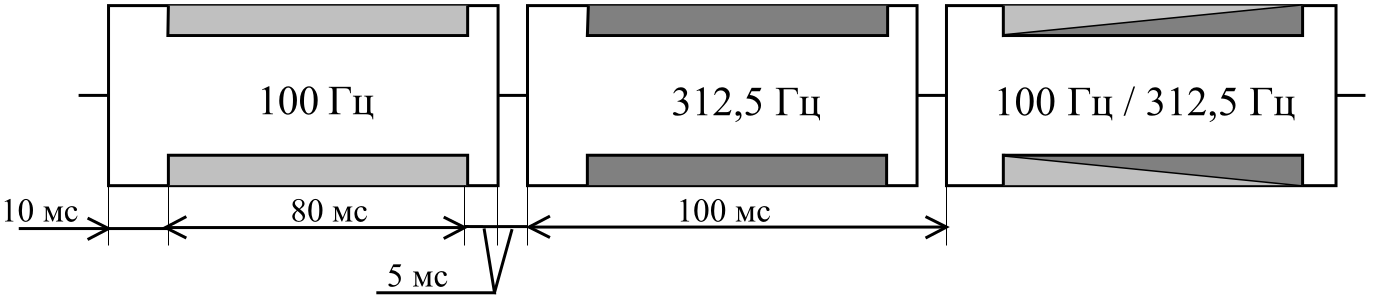
\includegraphics[width=0.5\textwidth]{dxxxw}
    \captionsetup{width=0.8\textwidth}
    \captionof{figure}{DXXXW signal fragment.}
    \label{fig:dxxxw}
\end{figure}

The RBU time code transmits
detailed time-related information, crucial for synchronization and timekeeping
across vast networks. The data structure includes:
\begin{enumerate}[noitemsep]
    \item \textbf{Time Code Elements:} year, month, day of the week, day of the
        month, hour, and minute, encoded in a binary-coded decimal (BCD)
        format, allowing receivers to decode the current date and time
        precisely.
    \item \textbf{DUT1 and dUT1 Corrections} that provide adjustments to UT1
        relative to UTC, catering for Earth's rotational irregularities.
    \item \textbf{Second and Data bits} which include unary encoding to
        indicate adjustments such as DUT1 values, enhancing the accuracy of
        timekeeping.
\end{enumerate}

Second markers are distinguished by a preceding 0.1-second interval modulated
at 312.5 Hz, while minute markers are identified by two consecutive 0.1-second
intervals prior to the second marker, each modulated at
312.5~Hz~\cite{vniiftri}. These modulation patterns allow accurate
determination of the second and minute boundaries in Coordinated Universal Time
(UTC).

\begin{figure}[H]
    \centering
    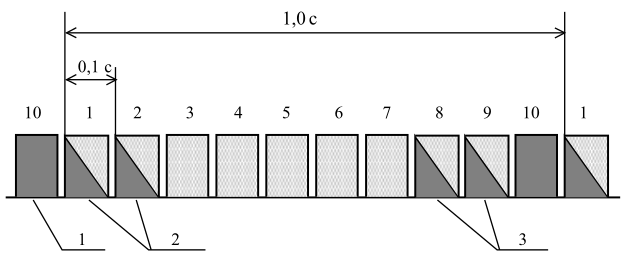
\includegraphics[width=0.6\textwidth]{dxxxw2}
    \captionsetup{width=0.8\textwidth}
    \captionof{figure}{RBU signal payload structure:\\ 1 -- Start-of-the-Second marker; 2 -- Information payload;\\ 3 -- Start-of-the-Minute marker.}
    \label{fig:dxxxw2}
\end{figure}

The RBU signal comprises two critical features aiding in accurate UTC time
phase determination:

\begin{enumerate}[noitemsep]
    \item The carrier wave undergoes brief interruptions for 5 ms every
        100 ms, denoted with empty space between bits of RBU signal payload on
        Figure~\ref{fig:dxxxw2}. These interruptions provide precise phase
        markers with ambiguity of 10.
    \item Additionally, a 312.5 Hz carrier modulation marks the beginning of
        each second, essential for resolving the phase ambiguity associated
        with the pulse per second (PPS) signal. These modulations are denoted
        with dark grey color rectangles indexed with number 10 on
        Figure~\ref{fig:dxxxw2}, while the light grey color illustrates 100 Hz
        modulations used to encode binary data which is irrelevant to the
        proposed approach.
\end{enumerate}



Notably, selection of the RBU radio station serves exclusively as a practical
example within this context. Other time signal stations, such as DCF-77
(Germany), WWWB (USA), and MSF (UK), are also operational globally.  The
optimal longwave time signal source for a specific application would be
determined through a comprehensive evaluation that considers factors such as
signal strength, propagation characteristics within the target deployment
region, and accessibility.  In essence, any longwave time signal station
located within suitable geographic proximity to the receiver could be
interchangeably employed within the proposed framework.

\subsubsection{Longwave Time Signal Range Limitations}

Investigations into the range limitations of longwave time signals are
essential for understanding their effective use in various applications.
Longwave (LW) signals, classified to encapsulate frequencies between 30 kHz and
300 kHz, are particularly suited for robust, long-distance transmission due to
their ability to follow the Earth's curvature via ground wave propagation. This
characteristic is instrumental in achieving extensive coverage, potentially
spanning national boundaries.

Conversely, despite these capabilities, the range of longwave signals can still be
constrained by several factors. Notably, the ionospheric conditions, which play
a crucial role in radio wave propagation, introduce variability in signal
reach. Solar activities, such as flares and sunspots, can significantly affect
ionospheric density and thus influence the propagation paths and stability of
longwave signals.

Furthermore, the topography and the electrical conductivity of the terrain over
which the signal travels can also impact its effective range. Areas with higher
conductivity, such as bodies of water or wetlands, can enhance ground wave
propagation, while rocky or mountainous regions may present challenges due to
signal absorption and scattering~\cite{longwave1,longwave2}.

Empirical studies, such as those referenced in ITU-R recommendations, suggest
that longwave time signals can reliably cover distances up to 2000 km under
optimal conditions. However, these theoretical ranges often require validation
through dedicated experimental research to confirm practical usability across
such expanses, especially in diverse geographic settings like Russia's vast
territories \cite{itur1997standard}.

In conclusion, while longwave time signals have inherent advantages for
wide-area coverage due to their propagation characteristics, their effective
range is not absolute and is influenced by a complex interplay of atmospheric,
topographical, and solar conditions. As such, continual monitoring and research
are necessary to optimize their application in global time and frequency
dissemination.

\subsubsection{Software Defined Radio}

Software Defined Radio (SDR) represents a transformative approach to radio
design, enabling radios to be extensively configured and controlled via
software. This technology allows for the replacement of traditional hardware
components, such as mixers and filters, with software processing. This shift
not only reduces physical constraints but also enhances the flexibility and
adaptability of radio systems to new frequencies and functionalities through
software updates.

A fundamental aspect of SDR technology is its reliance on in-phase (I) and
quadrature (Q) components to digitally represent radio frequency signals. These
components are essential for capturing all the information of a signal,
including its amplitude and phase. The I and Q components represent the signal
on orthogonal axes, with the I component aligned with the cosine wave and the Q
component aligned with the sine wave. This method offers several significant
advantages:

\begin{itemize}[noitemsep]
    \item \textbf{Complete Signal Representation:} I/Q data allows for the
        complete representation of a radio signal's phase and amplitude, which
        is crucial for accurately demodulating complex algorithms used in
        modern communication systems.
    \item \textbf{Improved Signal Integrity:} By processing signals in both the
        in-phase and quadrature dimensions, SDRs can more effectively
        distinguish between overlapping signals and reduce the likelihood of
        interference, leading to clearer and more reliable signal reception.
    \item \textbf{Flexibility in Signal Manipulation:} I/Q processing
        facilitates various signal manipulations such as shifting, modulation,
        and demodulation directly in the digital domain, offering extensive
        control over signal characteristics with high precision.
\end{itemize}

One of the critical applications of SDR technology is in GNSS spoofing, an area
of growing concern due to the potential security risks it poses. SDRs can
generate and transmit radio signals that mimic GNSS signals, making them
invaluable tools for both perpetrating and defending against spoofing attacks.
This capability allows security professionals and researchers to simulate
various spoofing scenarios to develop and test countermeasures that improve the
resilience of GNSS receivers. Effective anti-spoofing techniques, leveraging
the nuanced control offered by SDR, are vital for ensuring the security and
reliability of GNSS-dependent systems~\cite{hackrf1}.




\subsection{Methods}\label{sec:methods}

\subsubsection*{Literature Review and Theoretical Framework}

\begin{wrapfigure}{r}{0.5\textwidth}
    \centering
    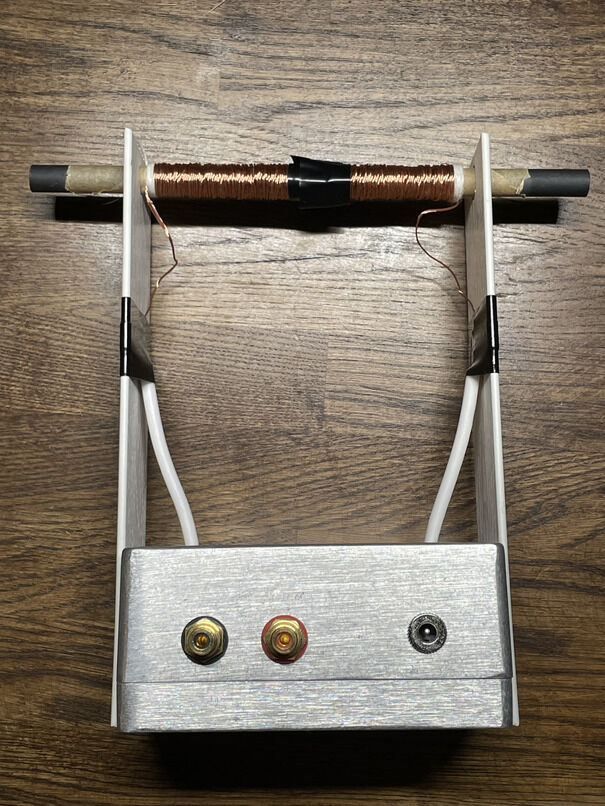
\includegraphics[width=0.4\textwidth]{my-antenna.jpg}
    \captionsetup{width=0.4\textwidth}
    \captionof{figure}{Active ferrite rod antenna with an integrated LNA.}
    \label{fig:my-antenna}
\end{wrapfigure}

The research commenced with a literature review focusing on the current
advancements and identified gaps in time synchronization technologies. This
review concentrated on the DVB-T and DVB-T2 standards, Precision Time Protocol
(PTP), and GNSS systems. The theoretical insights gained were pivotal in
guiding the experimental approach and highlighting the need for robust
synchronization solutions in Single Frequency Networks (SFNs).

\subsubsection*{Antenna Design and Signal Reception}

Critical to the experiment was the design and optimization of antennas for the
robust reception of longwave time signals. The setup included an active ferrite
rod antenna, seen on Figure~\ref{fig:my-antenna}. It is integrated with a
low-noise amplifier (LNA) to enhance the reception quality of the longwave
signals, essential for maintaining synchronization across SFN networks.

\subsubsection*{Experimental Setup}

The core of the experimental setup involved a hardware platform centered around
the STM32 microcontroller, known for its robust performance in real-time
applications. This platform was integral as a primary timing source to
synchronize SFN base stations, depicted in Figure~\ref{fig:setup-mess}.

\begin{figure}[H] \centering
    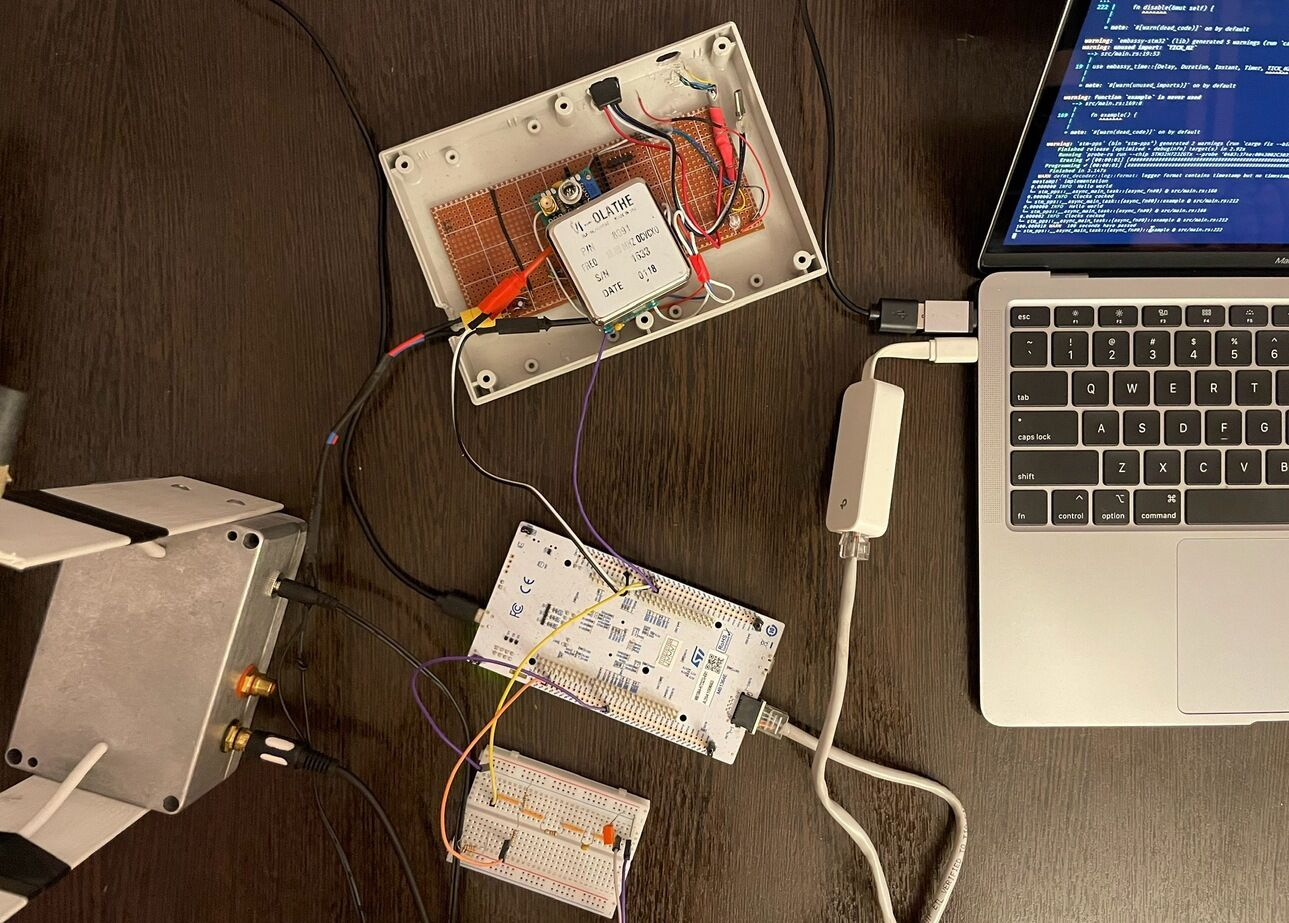
\includegraphics[width=0.7\textwidth]{setup-mess.jpg}
    \captionsetup{width=0.9\textwidth}
    \caption{Experimental setup showing key components: the STM32-NUCLEO
    development board at the center, the OCVCXO crystal at the top, the ferrite
    rod antenna on the left, and a workstation equipped with DSP algorithms on
    the right.}
    \label{fig:setup-mess}
\end{figure}

\subsubsection*{Digital Signal Processing and Algorithm Development}

Concurrently, novel Digital Signal Processing (DSP) algorithms were developed
to facilitate the extraction and interpretation of time signals from the
noise-laden data received by the antennas. These algorithms were crucial for
ensuring accurate time synchronization, particularly in challenging signal
environments. Furthermore, algorithms were developed to detect discrepancies in
GNSS and terrestrial-based time signals, enabling an internal switching
mechanism that maintains continuous synchronization of the SFN base stations.

\subsubsection*{System Integration and Testing}

The system's accuracy and reliability were further bolstered by integrating
oven-compensated voltage-controlled oscillators (OCVCXO). Known for their
stable signal output over time, these devices were instrumental in maintaining
synchronization precision. The entire setup's effectiveness was rigorously
validated through a series of empirical tests conducted under varied natural
conditions and at different distances from the radio time signal source.

\subsubsection*{Statistical Analysis of Phase Errors}

A key part of ensuring the reliability of time synchronization was the
statistical analysis of phase measurement errors. This involved verifying the
normality of the distribution of phase errors, which is critical for applying
certain statistical techniques. For precise measurements, the study employed
standard statistical formulas to determine the required sample size based on
the desired Standard Error of the Mean (SEM) to ensure the accuracy of
conclusions drawn from the data analysis.

\subsubsection*{GNSS Spoofing Resilience Evaluation}

To assess the time transfer framework's resilience against GNSS spoofing, an
SDR transmitter was used. The Great Scott Gadgets HackRF One, shown in
Figure~\ref{fig:hackrf}, was configured to simulate GNSS spoofing attacks to
evaluate the system's defensive mechanisms.

This methodological approach underscores our dedication to advancing SFN
synchronization technologies by addressing each component of the
synchronization process, from signal reception and processing to hardware
innovation and algorithmic development.

\begin{figure}[h]
    \centering
    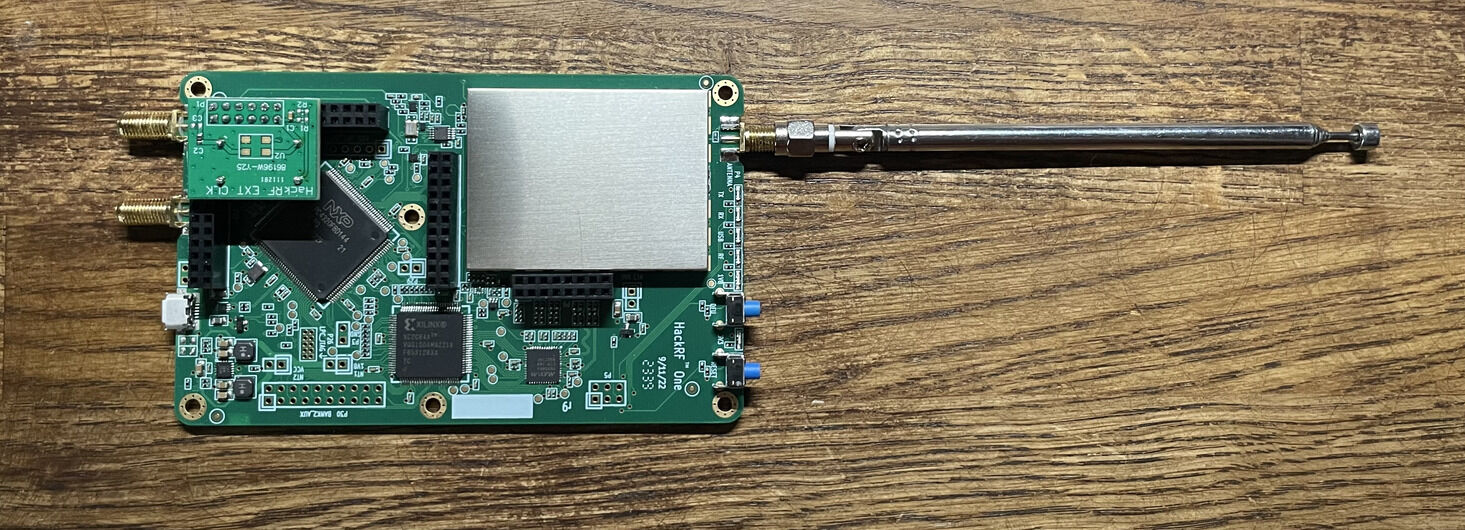
\includegraphics[width=0.7\textwidth]{hackrf.jpg}
    \caption{Great Scott Gadgets HackRF One with an RF shield.}
    \label{fig:hackrf}
\end{figure}



%This study initiates with a comprehensive literature review to contextualize
%the current advancements and gaps in time synchronization technologies, with a
%particular focus on the DVB-T and DVB-T2 standards, the Precision Time Protocol
%(PTP), and GNSS systems. This foundational understanding aids in framing the
%subsequent experimental inquiries.
%
%The experimental phase investigates the propagation characteristics of
%low-frequency radio signals, vital for developing a resilient synchronization
%framework. Antenna designs with varying characteristics are assessed to
%optimize the robust reception of these signals under diverse environmental
%conditions.
%
%Concurrently, novel Digital Signal Processing (DSP) algorithms are devised to
%enhance the extraction and interpretation of time signals from the noise-laden
%data received by the antennas. These algorithms are crucial for ensuring
%accurate time synchronization, especially in challenging signal environments.
%
%Central to the experimental setup is a hardware platform built around the STM32
%microcontroller, chosen for its robust performance and compatibility with
%real-time applications. This platform serves as a primary timing source to
%synchronize SFN base stations and is shown on Figure~\ref{fig:setup-mess}.
%
%\begin{figure}[h]
%    \centering
%    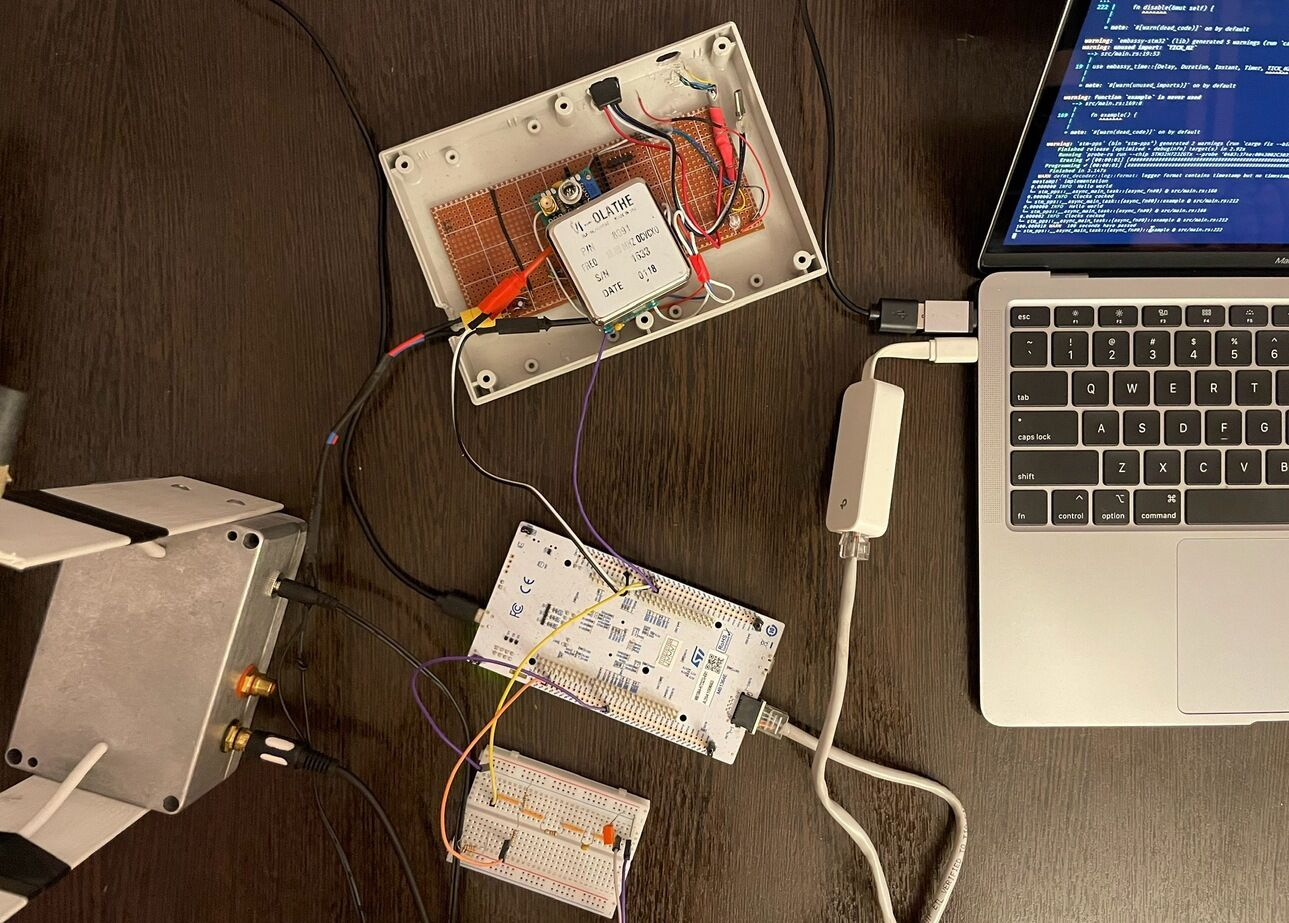
\includegraphics[width=0.6\textwidth]{setup-mess.jpg}
%    \captionsetup{width=0.9\textwidth}
%    \caption{Experimental setup showing key components: the STM32-NUCLEO
%    development board at the center, the OCVCXO crystal at the top, the
%    ferrite rod antenna on the left, and a workstation equipped with DSP
%    algorithms on the right.}
%
%    \label{fig:setup-mess}
%\end{figure}
%
%To further bolster the system's accuracy and reliability, especially during
%signal loss scenarios, the system integrates oven-compensated
%voltage-controlled oscillators (OCVCXO). Known for their stable signal output
%over time, these devices are instrumental in maintaining synchronization
%precision.
%
%The effectiveness of the entire setup is rigorously validated through a series
%of empirical tests, conducted under varied natural conditions and at different
%distances from the radio time signal source. These tests are essential for
%confirming the practical viability and robustness of the proposed
%synchronization system.
%
%Lastly, algorithms are developed to detect discrepancies in GNSS and
%terrestrial-based time signals. These algorithms enable an internal switching
%mechanism that maintains continuous synchronization of the SFN base stations,
%thus ensuring consistent broadcast quality.
%
%Time transfer framework resilience against GNSS spoofing is evaluated using an SDR transmitter
%
%\begin{figure}[h]
%    \centering
%    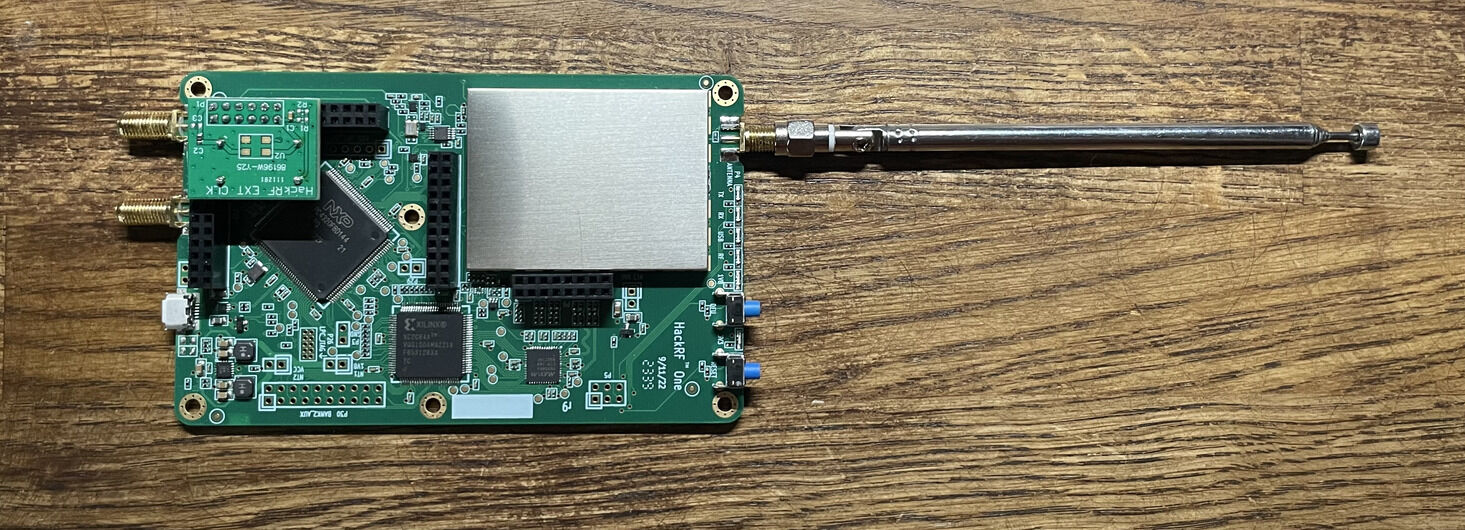
\includegraphics[width=0.7\textwidth]{hackrf.jpg}
%    \caption{Great Scott Gadgets HackRF One with an RF shield.}
%    \label{fig:hackrf}
%\end{figure}
%
%This methodological approach highlights our commitment to enhancing SFN
%synchronization technologies by addressing every component of the
%synchronization process, from signal reception and processing to hardware
%innovation and algorithmic development.
%
%\begin{figure}[h]
%    \centering
%    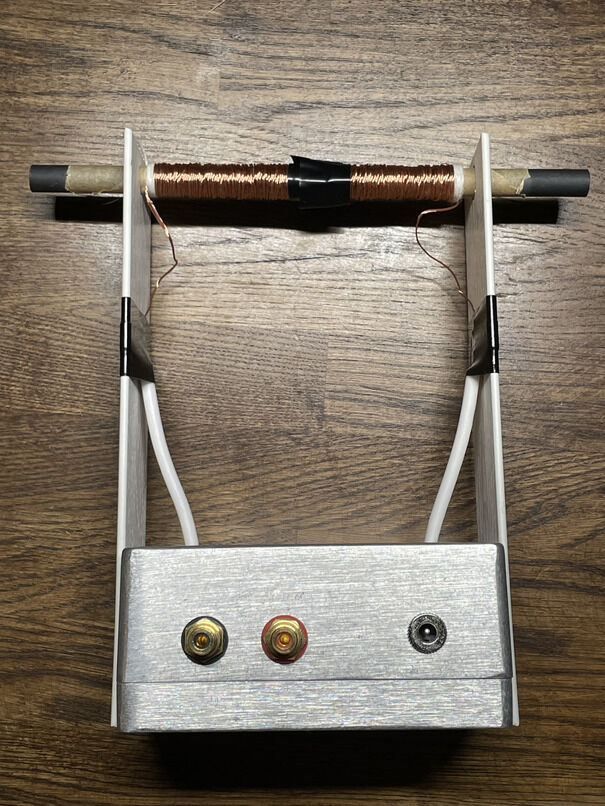
\includegraphics[width=0.4\textwidth]{my-antenna.jpg}
%    \captionsetup{width=0.8\textwidth}
%    \captionof{figure}{Active ferrite rod antenna with an integrated LNA.}
%    \label{fig:my-antenna}
%\end{figure}
%
%Figure~\ref{fig:my-antenna} depicts an active ferrite rod antenna
%integrated with a low-noise amplifier (LNA) to enhance signal reception.
%The antenna should be placed in an open area, away from potential sources of
%electromagnetic interference (EMI), and elevated if possible. Due to the
%directional sensitivity of the ferrite rod antenna, optimal signal reception is
%achieved when the rod is aligned perpendicular to the propagation vector
%of the RBU signal.


\pagebreak
\section{Time Transfer}\label{sec:time-transfer}

To design and evaluate resilient time transfer algorithms, it is imperative to
develop a robust and generalized time and frequency system. This system must
synchronize its time and frequency to Coordinated Universal Time (UTC) using
multiple GNSS constellations while incorporating a sufficiently stable clock
source to compensate for potential transient GNSS outages.

\subsection{Experimental Setup for PPS Synchronization}

In our experimental setup, the u-blox MAX-M10S GNSS receiver module serves as
the primary source of GNSS-synchronized Pulse-Per-Second (PPS) signals.
However, its internal Temperature-Compensated Crystal Oscillator (TCXO) lacks
the long-term stability required to maintain accurate timekeeping in
GNSS-deprived conditions~\cite{m10s-ds,m10s-im}.

To address the stability issue during periods of GNSS signal degradation (e.g.,
urban canyons, tunnels, jamming, or spoofing), this paper proposes a designed
generalized setup featuring an intermediate PPS source with enhanced long-term
stability. Specifically, we incorporate a 10 MHz Oven-Controlled
Voltage-Controlled Crystal Oscillator (OCVCXO) with a frequency tolerance of
0.1 ppm.

The intermediate stratum-1 PPS source is provided by an STM32 NUCLEO-H723ZG
development kit equipped with an Arm\textsuperscript{\textregistered}
\mbox{Cortex\textsuperscript{\textregistered}-M7} CPU~\cite{st-nucleo}. This development
kit is synchronized to the stable PPS signal generated by the u-blox MAX-M10S
module to correct the reference 10~MHz signal from the OCVCXO. The accurate and
reliable PPS signal locally-derived by STM32 from the OCVCXO enables
uninterrupted operation of DVB-T2 SFN transmitters, thereby mitigating service
degradation during GNSS signal outages.

\subsubsection{GNSS Module Configuration}\label{section:gnss-config}

The u-blox MAX-M10S GNSS receiver module is configured via a UART interface
using a proprietary UBX datagram protocol. The protocol features
commands such as \texttt{UBX-CFG-VALGET} and \texttt{UBX-CFG-VALSET} for
reading and modifying configuration parameters respectively~\cite{m10-id}.

To maximize accuracy at the expense of convergence speed, the receiver is
configured by modifying the following keys.

\begin{enumerate}[noitemsep]
    \item \texttt{CFG-NAVSPG-DYNMODEL = 0b0010}.
        To maximize accuracy, the receiver is configured in static positioning
        mode, given its stationary nature in this application.
    \item \texttt{CFG-SIGNAL-GLO\_ENA = 0b1} and \texttt{CFG-SIGNAL-BDS\_ENA = 0b1}.\\
        For improved precision and faster convergence, we enable GLONASS and BeiDou
        constellations, which are disabled by default.
    \item \texttt{CFG-RATE-MEAS = 0b1111101000}.
        A slower position update rate enhances stability and accuracy. We
        configure the measurement rate of 0.1~Hz as it is not crucial for the
        scenario of time transfer.
    \item \texttt{CFG-RATE-TIMEREF = 0b000}.
        Different GNSS constellations utilize distinct time systems. This
        configuration allows us to align PPS measurements to Coordinated
        Universal Time (UTC)~\cite{m10s-im}. This way multiple GNSS receivers
        from different vendors in an SFN will consistently output universally
        synchronized PPS.
\end{enumerate}

To monitor the GNSS receiver's operational status, the \texttt{UBX-MON-COMMS} key can be
configured to output a stream of NMEA, RTCM, SPARTN, and UBX datagrams. These
datagrams contain comprehensive information about location, speed, time, signal
spectrum, tracked satellites, satellites in view, carrier-to-noise density
ratios (C/N\textsubscript{0}), Position Dilution of Precision (PDOP), and
other metrics~\cite{m10-id}. The data can be visualized using the PyGPSClient GUI
application, as shown in Figure~\ref{fig:pygpsclient-fix}~\cite{pygpsclient}.

\begin{figure}[H]
    \centering
    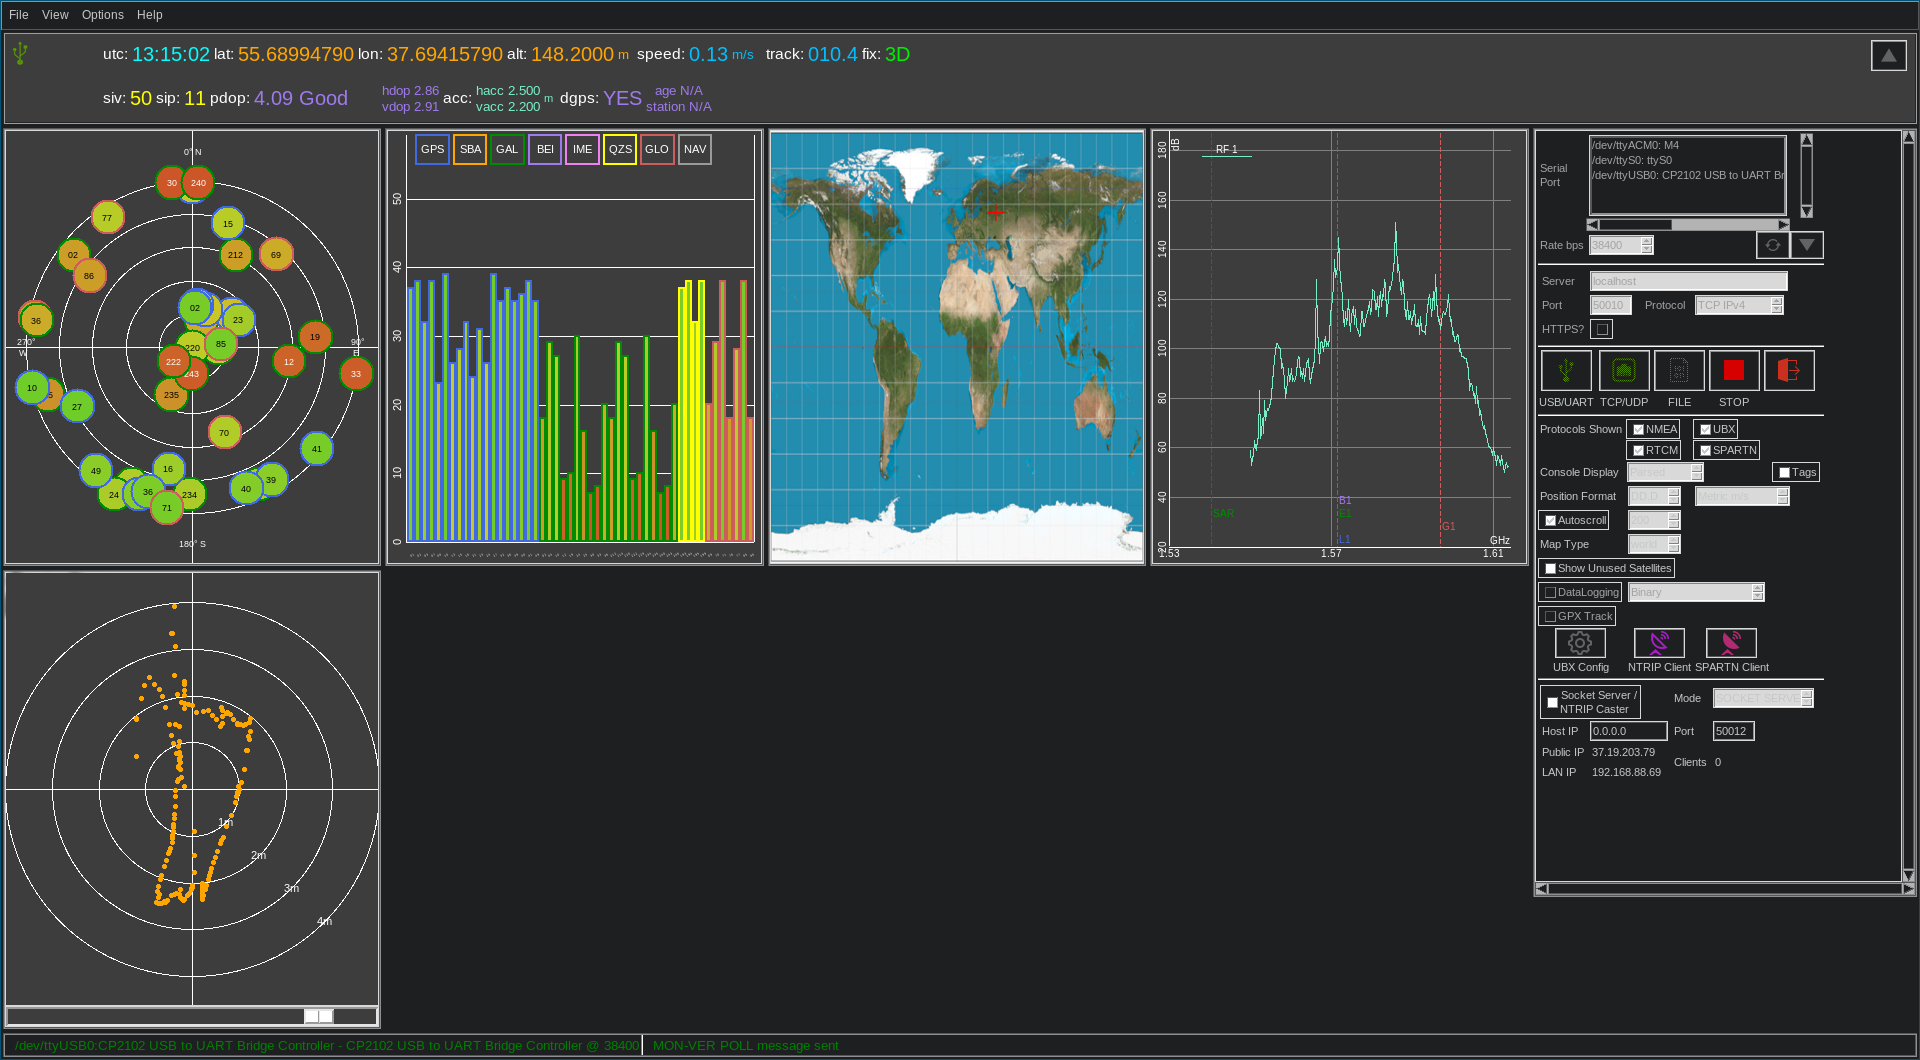
\includegraphics[width=0.7\textwidth]{pygpsclient}
    \captionsetup{width=0.8\textwidth}
    \captionof{figure}{PyGPSClient displaying the operational status of the u-blox MAX-M10S GNSS receiver.}
    \label{fig:pygpsclient-fix}
\end{figure}

After obtaining a position fix, the output PPS signal from the GNSS receiver
can be verified using a logic analyzer. The signal should exhibit a period of 1
Hz with a duty cycle of 10\%. Figure~\ref{fig:pps-dsview} shows the PPS signal
as visualized in DSView, a digital oscilloscope software~\cite{dsview}. An
error of 1.7 microseconds can be observed in period calculation, as
caused by sample rate.

\begin{figure}[h]
    \centering
    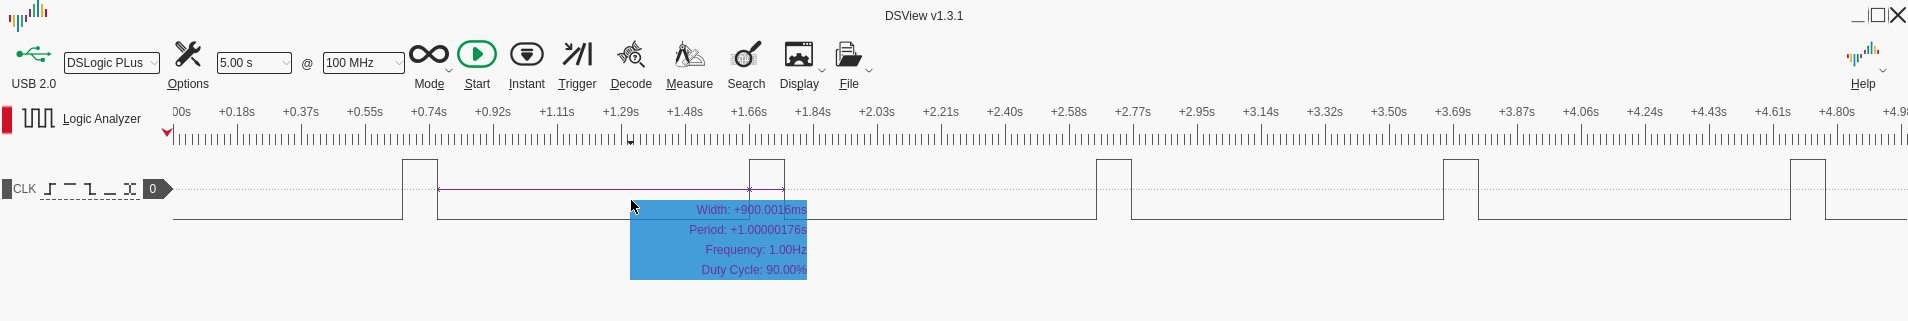
\includegraphics[width=0.9\textwidth]{dsview}
    \captionsetup{width=0.8\textwidth}
    \captionof{figure}{Representation of the PPS signal in DSView digital oscilloscope software.}
    \label{fig:pps-dsview}
\end{figure}

\subsubsection{PPS Registration with STM32}\label{sec:stm-pps-basic}

To achieve highly consistent latency between the PPS pulse generation on the
GNSS receiver module and its registration on the STM32 microcontroller, careful
hardware design is essential. One effective approach is to route the PPS signal
to a General Purpose Input/Output (GPIO) pin configured as an input with a
pull-down resistor. This pin can then be assigned to the External
Interrupt/Event (EXTI) controller~\cite{stm-ds}. By setting the EXTI controller
to trigger on the rising edge of the PPS signal, a hardware interrupt is
dispatched with a configurable priority, allowing precise PPS pulse registration
on the STM32~\cite{stm-pm}.

\subsection{OCVCXO Frequency Correction}

Crystal oscillator accuracy and precision are susceptible to variations in
current, temperature fluctuations, vibration-induced noise, physical aging,
ambient pressure, humidity, and electromagnetic fields~\cite{xo-stability}. To
compensate for these factors, Voltage-Controlled Crystal Oscillators (VCXOs)
employ a Phase-Locked Loop (PLL) circuits with frequency multipiers. By varying
the voltage supplied to the PLL pin, the oscillator's frequency can be
adjusted. The STM32H7 MCU provides multiple 12-bit Digital-to-Analog Converters
(DACs) that allow precise voltage control via DAC peripheral hardware
registers~\cite{stm-ds}.

To accurately measure the error of the OCVCXO, the number of clock cycles it
generates between two consecutive PPS pulses must be determined. The STM32H7's
Reset and Clock Controller (RCC) provides a feature that facilitates this
measurement. The RCC manages several internal clock sources, including a
high-speed internal 64 MHz oscillator (HSI), low-power internal 4 MHz
oscillator (CSI), accurate 48 MHz oscillator and a low-speed internal 32 kHz RC
oscillator (LSI). The RCC also supports high-speed external oscillators (HSE)
ranging from 4 to 48 MHz. The clock security system automatically switches to
the HSI if a loss of the external clock is detected~\cite{stm-ds}.

This paper proposes wiring the OCVCXO as the HSE of the STM32 and connecting
the GNSS receiver's PPS signal to a GPIO input pin. An interrupt should be
configured with the highest priority, as described in
Section~\ref{sec:stm-pps-basic}, to register the PPS signal. An interrupt
handler can then be programmed to follow this algorithm:

\begin{enumerate}[noitemsep]
    \item \textbf{Capture Cycle Count}: \\
        Read the value of the CPU Cycle Counter (CYCCNT) from the
        data watchpoint and trace unit (DWT) cycle count register~\cite{stm-rm}.
    \item \textbf{Compute the difference} between the current and previously captured
        CYCCNT values to determine the number of CPU cycles elapsed since the
        last interrupt.
    \item \textbf{Adjust PLL Voltage}:
        \setlist{nolistsep}
        \begin{itemize}[noitemsep]
        \item If the difference is greater than 10 million cycles, reduce
            the PLL voltage via the DAC, as the clock runs too fast.
        \item If the difference is less than 10 million cycles, increase
            the PLL voltage to speed up the clock, as the clock runs too slow.
    \end{itemize}
\end{enumerate}

The accumulated difference in cycles can be used instead to account for the PLL
convergence delay. A reference algorithm that accumulates the error over 100
PPS pulses is provided in Appendix~\ref{appendix:interrupt-algo}.

\subsection{PPS Phase Synchronization}

Once the frequency stability of the Oven-Controlled Voltage-Controlled Crystal
Oscillator (OCVCXO) has been calibrated and corrected, the next imperative is
to develop a strategy for generation of a synchronized Pulse-Per-Second (PPS)
signal. This synchronization ensures temporal coherence between the local time
signal source and Coordinated Universal Time (UTC).

A straightforward hardware solution involves utilizing frequency division
circuitry via a sequence of binary counters, such as the Texas Instruments
CD4040 series~\cite{cd4040}. By setting a division factor of 10 million and
providing an input from the OCVCXO clock, the carry-out signal from the final
counter generates a stable 1 Hz output. To align this signal phase with the PPS
output from the GNSS receiver, the GNSS PPS signal is routed to the reset pins
of the binary counters. Consequently, the locally generated PPS signal
maintains phase alignment with the GNSS PPS signal, thereby aligning with UTC
through a cost-effective hardware solution.

However, this approach exhibits notable limitations, primarily the lack of
configurability in phase offsets to account for time signal propagation errors.
In contrast, the STM32 H7 MCU series offers integrated high-resolution timers
that, when configured in pulse-width modulation (PWM) mode, can function as
versatile frequency dividers. By dynamically adjusting the PWM duty cycle and
precisely timing resets via software, it is possible to generate an accurate
PPS signal with user-configurable phase offsets, thus providing more precise
temporal synchronization~\cite{stm-timer}.

To evaluate the generated PPS signal's temporal precision with respect to the
reference GNSS signal, a methodology for capturing the relative phase offset
between the two signals is necessary. While monitoring a generated a PPS signal
with picosecond-level precision typically requires sophisticated
instrumentation, monitoring the phase difference without signal generation is
achievable with readily available microcontroller peripherals.

A detailed interrupt-driven approach to capture and monitor the phase offset
between the OCVCXO-derived PPS and GNSS-derived PPS signals is outlined in
Appendix~\ref{appendix:interrupt-algo} on line 38. The algorithm involves
accumulating phase error measurements across multiple PPS pulses, thereby
mitigating transient inaccuracies and enabling long-term, high-stability
synchronization.

A detailed interrupt-driven approach to capture and monitor the phase offset
between the OCVCXO-derived PPS and GNSS-derived PPS signals is outlined in
Appendix~\ref{appendix:interrupt-algo}. The algorithm involves accumulating
phase error measurements across multiple PPS pulses, thereby mitigating
transient inaccuracies and enabling long-term, high-stability synchronization.

\subsection{Results Overview}

A comprehensive time transfer experiment was conducted over a span of 13,000
seconds (approximately 3.6 hours), during which multiple metrics pertaining to
the Oven-Controlled Voltage-Controlled Crystal Oscillator (OCVCXO) were
recorded. The experiment began with a cold-start of the GNSS receiver and the
OCVCXO at room temperature, providing a full view of the crystal's warm-up
phase and subsequent stabilization.

For the evaluation, key metrics such as the phase and frequency of the oscillator were analyzed. The phase was calculated using the formula:
\[
    \phi(T_{\text{interrupt}}) = f(T_{\text{interrupt}}) \mod 10000000
\]
where $f(T)$ is the value of the CYCCNT cycle count register at time $T$.

\begin{figure}[H]
  \centering
  \begin{subfigure}[b]{0.48\textwidth}
    \centering
    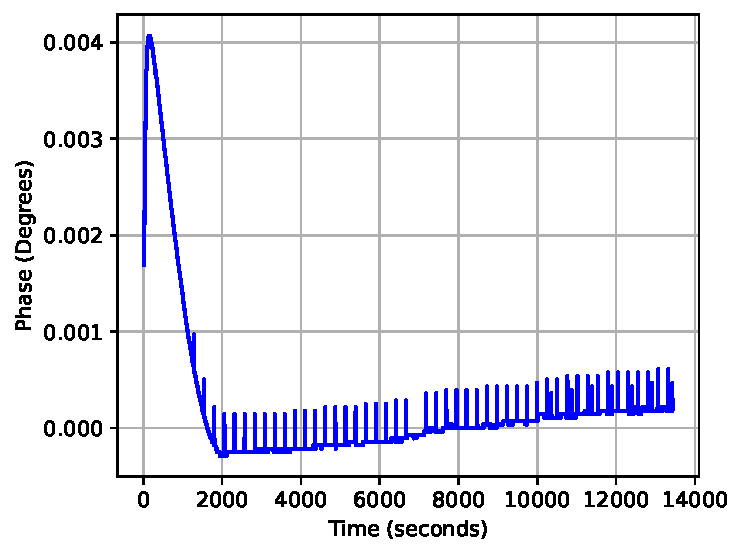
\includegraphics[height=0.7\textwidth]{phase-deg-raw.pdf}
    \caption{Unfiltered}
    \label{fig:phase-deg-raw}
  \end{subfigure}
  \hfill
  \begin{subfigure}[b]{0.48\textwidth}
    \centering
    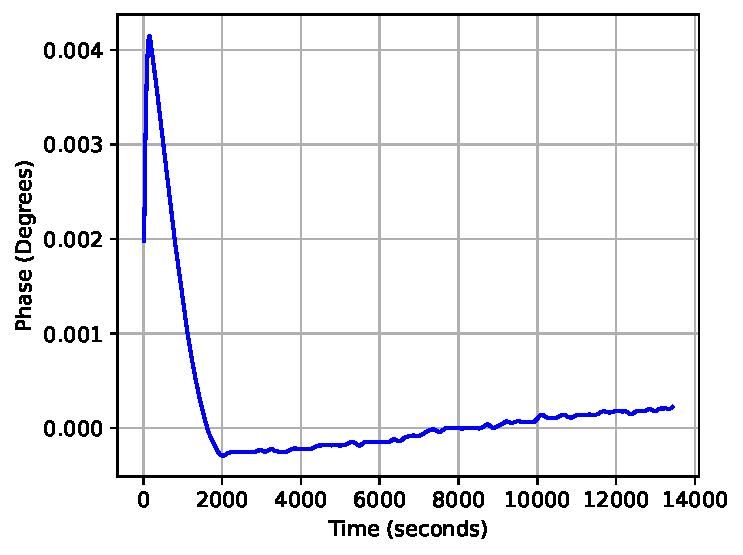
\includegraphics[height=0.7\textwidth]{phase-deg-smooth.pdf}
    \caption{Smoothed with Savitzky-Golay}
    \label{fig:phase-deg-smooth}
  \end{subfigure}
  \captionsetup{width=0.8\textwidth}
  \caption{Relative OCVCXO observed phase value over time.}
  \label{fig:phase-val}
\end{figure}

The warm-up phase of the OCVCXO is observed during the initial 2,000 seconds,
as depicted in Figure~\ref{fig:phase-deg-raw}. During this interval,
significant frequency drift is noticeable due to thermal effects as the
crystal's oven stabilizes. The cumulative frequency error and phase offset
stabilize gradually as the crystal reaches its operating temperature.

\begin{wrapfigure}{r}{0.5\textwidth}
    \centering
    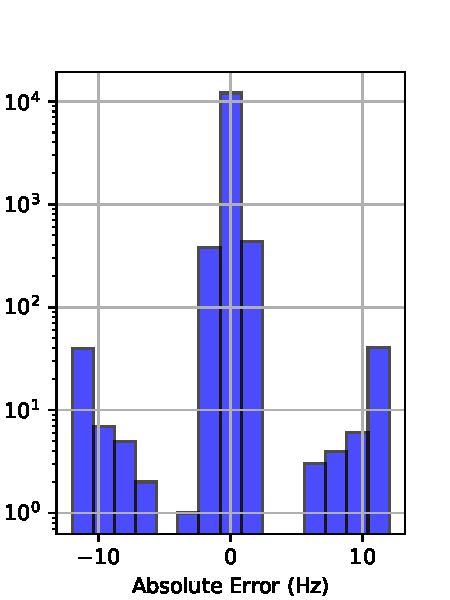
\includegraphics[width=0.4\textwidth]{err-bins.pdf}
    \captionsetup{width=0.4\textwidth}
    \caption{OCVCXO frequency offsets distributions with two peaks at $\pm 10$~Hz, caused by PPS signal debounce.}
    \label{fig:err-bins}
\end{wrapfigure}

After the warm-up period, periodic noise in the form of 10 Hz jumps is visible
in the raw phase data (Figure~\ref{fig:phase-deg-raw}) and in the histogram of
instantaneous frequency offset values (Figure~\ref{fig:err-bins}). These jumps
are attributed to debounce effects in the GNSS PPS signal and software
interrupt latencies, representing measurement artifacts rather than inherent
issues with the OCVCXO. To mitigate this noise, a Savitzky-Golay filter was
applied, producing a smoothed frequency stability profile
(Figure~\ref{fig:phase-deg-smooth}) and cumulative relative frequency error
(Figure~\ref{fig:cumsum-err-smooth}).

The Savitzky-Golay filter is a digital smoothing filter that applies a
polynomial fitting over a sliding window to preserve important features like
peak heights and widths while reducing noise. The polynomial coefficients are
computed using the least-squares method. For a given window size \( N \) and
polynomial order \( k \), the smoothed value \( y_i' \) of data point \( y_i \)
is calculated as:
\[
y_i' = \sum_{j=-m}^{m} c_j y_{i+j}
\]
where:
\( m = \frac{N-1}{2} \), and
\( c_j \) are the filter coefficients derived from polynomial fitting~\cite{sg-filter}.

In this experiment, a window size of 301 samples and a polynomial order of 3
were chosen to balance the trade-off between noise reduction and curve shape
distortion.


The smoothed results highlight the OCVCXO's frequency stability over the entire
duration of the experiment, with a frequency change of 10 Hz over 11,000
seconds post-warmup. The relative frequency error is 0.09 parts per billion
(ppb), calculated as:
\[
    \frac{10\ \text{Hz}}{11000 \cdot 10 \text{MHz}} = 9 \times 10^{-11} \approx 0.09\ \text{ppb}
\]

Simultaneously, phase stability achieved a drift of $6 \times 10^{-4}$ degrees, equivalent
to approximately 2 microseconds, over the same period.

The linear downward trend in cumulative relative frequency error suggests that
the OCVCXO was oscillating $0.0009$~Hz below the target 10 MHz frequency, with
the limited 12-bit resolution of the Digital-to-Analog Converter (DAC) unable
to fully compensate. Despite this, the observed frequency stability remains
within operational margins for SFN applications~\cite{1dvbt2, 2dvbt2, 3dvbt2, 4dvbt2, morshed2009synchronization}.


These results do not account for the drift of the GNSS receiver's internal
Temperature-Compensated Crystal Oscillator (TCXO), which could impact the
accuracy of the measurements. Comprehensive validation of this experimental
setup requires precision instrumentation, such as geodetic antennas with GNSS
phase-locking capability~\cite{geodesic,gps-time-transfer}.

\begin{figure}[H]
    \centering
    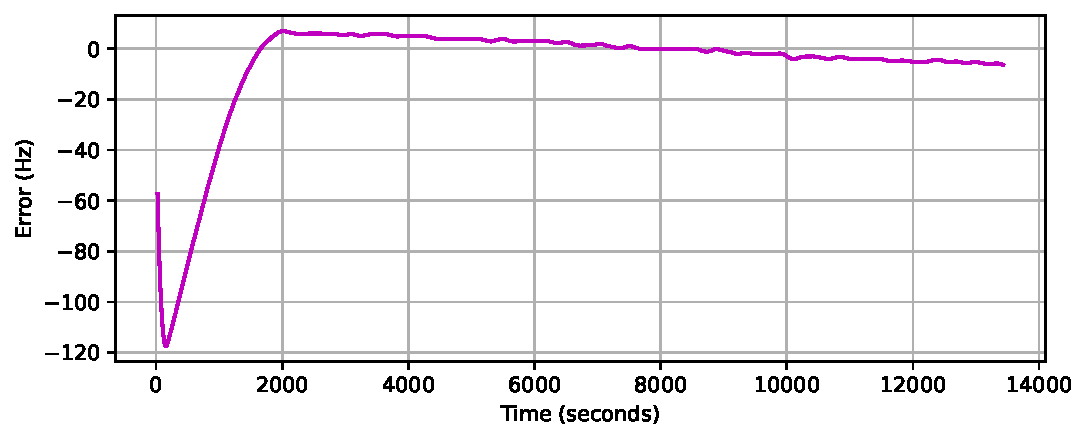
\includegraphics[width=0.7\textwidth]{cumsum-err-smooth.pdf}
    \captionsetup{width=0.8\textwidth}
    \caption{Cumulative relative OCVCXO observed frequency error smoothed with Savitzky-Golay filter.}
    \label{fig:cumsum-err-smooth}
\end{figure}

\subsection{Conslusions}

In summary, this foundational time transfer experiment demonstrated the
efficacy of OCVCXO frequency correction and PPS phase synchronization using
STM32 microcontrollers. The subsequent section addresses resilient time
transfer in the context of GNSS spoofing, introducing innovative algorithms and
methodologies to maintain synchronization accuracy despite intentional
interference.

With a foundational time transfer setup in place, the next section focuses on
enhancing time transfer resilience, particularly against GNSS spoofing. Here,
this paper delves into innovative algorithms and methodologies designed to
maintain accurate and reliable synchronization despite the presence of
intentional signal interference.

\pagebreak
\section{Resilient Time Transfer}\label{sec:resilient-time-transfer}

The resilience of time transfer is paramount for reliable GNSS-based services
due to the increasing vulnerability of these services to spoofing and
interference attacks. The proposed framework for resilient time transfer relies
on incorporating diverse timing sources and validating the consistency of
GNSS-derived timing through cross-checking methodologies with alternative
references, following the principles outlined by Zhang et al. in ``Protecting
GNSS-based Services using Time Offset Validation''~\cite{time-offset,celllocate}.

\subsection{Concept overview}

To improve resilience against spoofing attacks, an effective time
cross-checking method must be developed using alternative timing sources,
specifically focusing on absolute and relative time validation. This section
explores and refines methodologies to enhance GNSS-based time transfer
resilience using external time sources, with specific emphasis on detecting
intentional time shifts.

The validation framework proposed by Zhang et al. involves two primary strategies:

\begin{enumerate}
    \item \textbf{Absolute Time Validation:}
        By comparing the absolute difference between GNSS-provided time and an alternative source:
        \[
            f(t) = f(|T_{\text{ext}}(t) - T_{\text{GNSS}}(t)|)
        \]
        where $T_{\text{ext}}$ represents the time from an external source and
        $T_{\text{GNSS}}$ denotes the GNSS-derived UTC time.
        The result is then compared to the accuracy threshold of the external source, $\varepsilon_{\text{ext}}$.

    \item \textbf{Relative Time Validation:}
        This method examines the difference in elapsed time between consecutive GNSS-provided intervals:
        \[
            f(t) = f(|\Delta T_{\text{ext}}(t) - \Delta T_{\text{GNSS}} (t) |)
        \]
        where $\Delta T_{\text{ext}}$ and $\Delta T_{\text{GNSS}}$ represent the
        elapsed intervals of external and GNSS time, respectively.
\end{enumerate}

This paper advocates for the incorporation of an alternative time source
derived from a longwave time signal and standard-frequency radio station into a
resilient time transfer framework. The specific station under consideration is
the RBU facility operating near Moscow, Russia.

Longwave radio transmissions offer several advantages as a time reference. They
demonstrate superior penetration capabilities through dense urban environments
compared to GNSS signals~\cite{itu2007ground}. Additionally, the physics of radio wave
propagation at these frequencies makes them demonstrably less susceptible to
spoofing attacks~\cite{classen2013jamming}.

To achieve resilient time transfer with RBU radio time signal, the following steps are undertaken:

\begin{enumerate}[noitemsep]
    \item \textbf{Antenna Setup:}
        An antenna designed and tuned to the $66.\overline{6}$ kHz frequency of the RBU
        signal should be employed to maximize reception quality.

    \item \textbf{Signal Processing Algorithm:}
        Digital signal processing algorithms are proposed to extract
        relative timing information from the RBU signal to supplement GNSS-based
        timing:

    \begin{enumerate}[noitemsep]
        \item \textbf{Preprocessing:}
        Filter and demodulate the received longwave signal to reduce noise and interference.

        \item \textbf{Clock Recovery and Decoding:}
        Extract the timing markers and calculate the time signal phase.

        \item \textbf{Time Offset Calculation:}
        Compare the RBU time phase with the UTC time phase to compute the time offset.
    \end{enumerate}

    \item \textbf{Time Cross-Checking and Validation:}
        The time offset between the GNSS and RBU signals is monitored over
        a rolling window to detect discrepancies. A threshold is set
        based on the accuracy of the RBU signal to flag spoofing attempts
        and disable time transfer with the compromised GNSS receiver.
\end{enumerate}

For illustrative purposes, Figure~\ref{fig:device} depicts a time and frequency
transfer system. The system comprises a stratum-1 time and frequency signals
source, realized by an STM32 development board driven by a High-Speed External
(HSE) clock in the form of an Oven-Controlled Voltage-Controlled Crystal
Oscillator (OCVCXO). Additionally, it includes a u-blox MAX-M10S GNSS receiver
module, an RBU antenna, and a personal computer configured for digital signal
processing of the digitized signal received from the RBU-tuned antenna.

\begin{figure}[t]
    \centering
    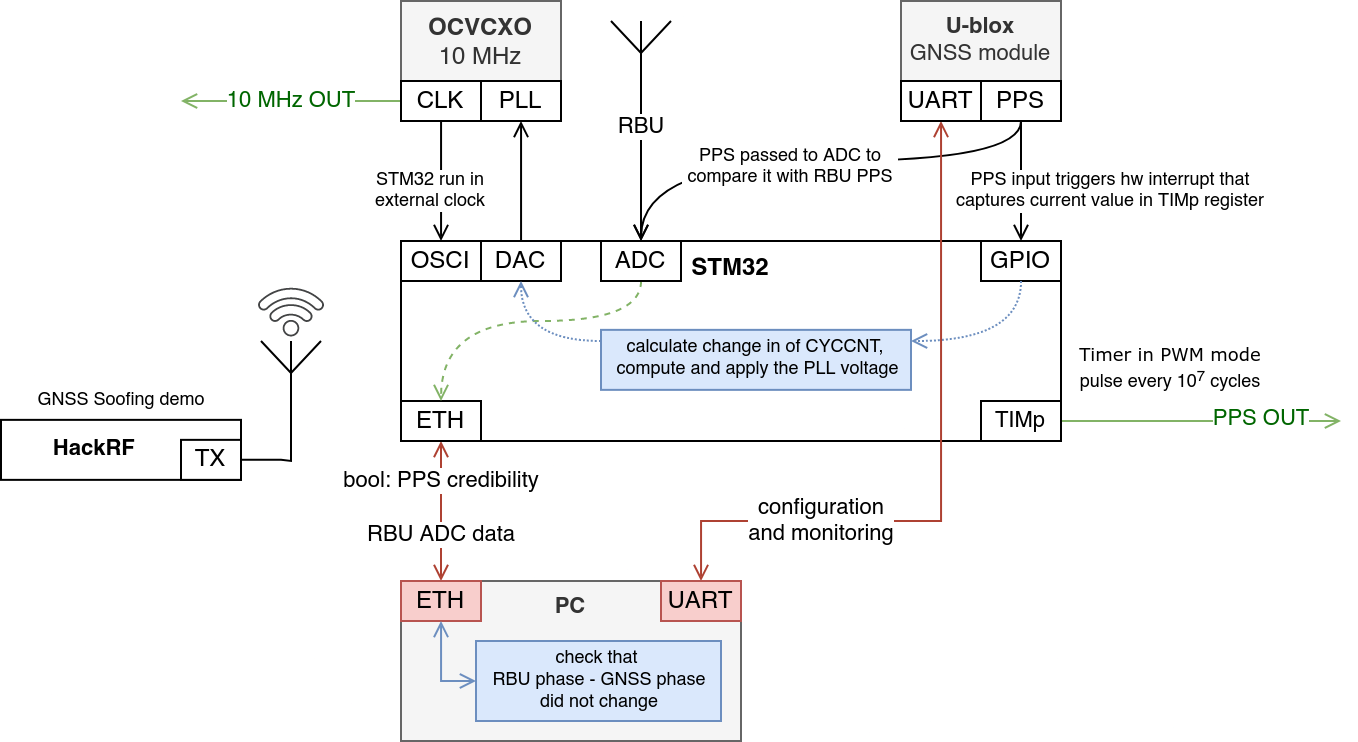
\includegraphics[width=0.9\textwidth]{device}
    \captionsetup{width=0.8\textwidth}
    \captionof{figure}{Resilient time and frequency transfer system schematic
    outlining proposed hardware and software architecture.}
    \label{fig:device}
\end{figure}

To facilitate system performance evaluation under GNSS spoofing conditions, a
Software Defined Radio (SDR) HackRF One transmitter is employed to simulate a GPS
constellation signal in Section~\ref{sec:hackrf}.

\subsection{RBU Signal Processing}

\subsubsection{Antenna Construction}

Historically, longwave time signals have been received using ferrite rod
antennas, a design often employed in wristwatches and other portable
devices~\cite{time-measurement}. These antennas are constructed with a ferrite
bar wrapped in a conductive wire.

For effective reception of the RBU longwave time signal at $66.\overline{6}$
kHz, an antenna specifically designed and tuned to this frequency is required.
The ferrite rod antenna offers high selectivity and signal sensitivity due to
the ferrite core's magnetic properties, which concentrate the magnetic flux and
enhance signal reception.

A ferrite rod antenna suitable for receiving the RBU signal typically has the
following specifications~\cite{antennas}:

\begin{itemize}[noitemsep]
    \item \textbf{Ferrite Rod Dimensions:} The rod should be 100-150 mm in
        length and 10-12 mm in diameter. A ferrite material with high
        permeability (\(\mu\)) is recommended, such as N48 or N87, to enhance
        signal sensitivity.
    \item \textbf{Wire Gauge:} Enamel-coated copper wire (magnet wire) of
        0.1-0.2 mm in diameter.
    \item \textbf{Number of Loops:} 100-200 turns around the ferrite rod to
        achieve resonance at $66.\overline{6}$ kHz.
\end{itemize}

The inductance (\(L\)) of the coil is calculated using:
\[
L = \frac{\mu_0 \mu_r A N^2}{l}
\]
where:
 \( \mu_0 \) is the permeability of free space (\(4\pi \times 10^{-7}\) H/m),
 \( \mu_r \) is the relative permeability of the ferrite material,
 \( A \) is the cross-sectional area of the ferrite rod,
 \( N \) is the number of turns,
 \( l \) is the length of the coil.

The resonant frequency (\(f\)) of the antenna is determined using
the following formula:
\[
f = \frac{1}{2\pi \sqrt{L C}}
\]
where \( L \) is the inductance of the coil, and \( C \) is the capacitance of
the tuning capacitor.
To tune the antenna to the RBU signal frequency, a parallel capacitor \(C\)
is selected to resonate at $66.\overline{6}$ kHz.


\subsubsection{Experimental Validation of Antenna Performance}\label{section:antenna-recv}

To quantitatively assess the efficacy of the proposed longwave time signal
reception strategy, field measurements were conducted at two geographically
distinct locations: Moscow, Russia (in close proximity to the RBU transmitter),
and Saint Petersburg, Russia (approximately 600 kilometers apart). The
rationale behind this experiment design was to evaluate the signal degradation
over a varying propagation distance.

Wavelet analysis, a time-frequency signal processing technique, was employed to
characterize the spectral properties of the received RBU signal at both
locations. Wavelet transforms decompose a signal into its constituent
time-frequency components, enabling the visualization of both signal frequency
content and its variation over time. This analysis method is particularly
well-suited for non-stationary signals, such as the RBU transmission which
incorporates timing markers superimposed on a carrier wave.

The wavelet power spectra for the RBU signal received in Moscow and Saint
Petersburg are presented in Figures~\ref{fig:moscow-spectrum}
and~\ref{fig:spb-spectrum}, respectively. As anticipated, the signal exhibits a
dominant spectral component at the expected RBU carrier frequency of
$66.\overline{6}$~kHz.

\begin{figure}[h]
  \centering
  \begin{subfigure}[b]{0.48\textwidth}
    \centering
    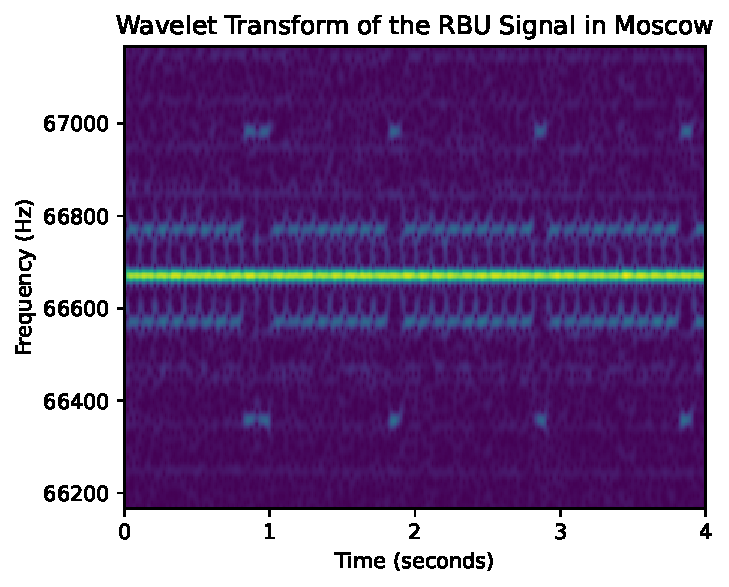
\includegraphics[height=0.75\textwidth]{ant-moscow.pdf}
    \caption{Moscow}
    \label{fig:moscow-spectrum}
  \end{subfigure}
  \hfill
  \begin{subfigure}[b]{0.48\textwidth}
    \centering
    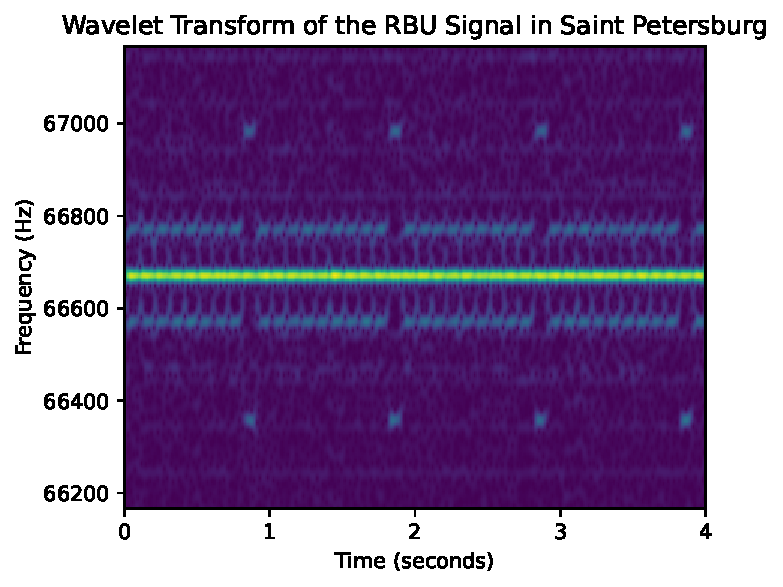
\includegraphics[height=0.75\textwidth]{ant-spb.pdf}
    \caption{Saint Petersburg}
    \label{fig:spb-spectrum}
  \end{subfigure}
  \captionsetup{width=0.8\textwidth}
  \caption{Wavelet transform of the RBU signal recorded at different distances from the transmitter.}
\end{figure}

Encouragingly, the wavelet power spectra for both recordings reveal minimal
spectral noise or interference across the frequency band of interest,
signifying successful reception and demodulation of the RBU signal. Furthermore,
the presence of a clear and well-defined time-domain marker within the Moscow
recording (Figure~\ref{fig:moscow-spectrum}, near the one-second time mark)
underscores the viability of extracting timing information from the received
signal using the proposed digital signal processing algorithms.

The successful reception and characterization of the RBU signal at both test
locations, even across a substantial propagation distance, validates the
potential of incorporating longwave time signal references into a resilient
GNSS time transfer framework. Following efforts will concentrate on the
development and implementation of robust digital signal processing algorithms
to extract timing information from the RBU signal for time transfer
applications.

\subsubsection{ADC Circular Buffer DMA Configuration}

The STM32 H7 microcontroller series incorporates multiple 16-bit
Analog-to-Digital Converters (ADCs) that can be extended to 16-bit resolution
via sigma-delta modulation. To facilitate continuous signal acquisition with
minimal computational overhead, the integrated Direct Memory Access (DMA)
peripheral is configured in Circular mode. This allows seamless data transfer
from the ADC to memory while minimizing CPU involvement.

DMA enables efficient data transfer by offloading memory transactions from the
CPU, thus allowing uninterrupted signal acquisition. In Circular mode, the DMA
controller automatically wraps around to the initial memory address once the
end of the buffer is reached, forming a circular buffer that continuously
stores new ADC data. The key configuration parameters include:

\begin{enumerate}[noitemsep]
    \item \textbf{Source and Destination Addresses:} Defines the ADC data
        register as the source and a pre-allocated memory buffer as the
        destination.
    \item \textbf{Transfer Size:} Specifies the number of data elements to be
        transferred per DMA transaction.
    \item \textbf{Increment Modes:} Configures the source as non-incremental
        and the destination as incremental to support circular buffering.
    \item \textbf{Circular Mode Activation:} Enables automatic wrapping to the
        beginning of the buffer.
\end{enumerate}

The Circular mode ensures continuous signal acquisition without data loss while
minimizing the load on the CPU, which only needs to configure the DMA transfer.

The STM32 H7 ADCs offer multiple conversion modes to accommodate various signal
acquisition needs:

\begin{enumerate}[noitemsep]
    \item \textbf{Single:} Converts a single input channel, operating in
        single-shot or continuous mode.
    \item \textbf{Scan:} Converts a predefined set of input channels in
        single-shot or continuous mode.
    \item \textbf{Discontinuous:} Converts a subset of predefined input
        channels at each trigger signal.
\end{enumerate}

For this resilient time transfer application, this paper proposes adoption of
Single Mode with continuous conversion to monitor a single RBU signal channel.
This approach ensures consistent signal acquisition with minimal overhead,
providing the data required for robust time validation.

The ADC-to-DMA data transfer mechanism proposed by this paper operates as follows:

\begin{enumerate}[noitemsep]
    \item \textbf{ADC Conversion:} The ADC continuously converts the analog
        signal to a digital representation and stores the result in its data
        register.
    \item \textbf{DMA Transfer into memory:} The DMA controller autonomously transfers the
        ADC result to a circular buffer in memory.
    \item \textbf{Transfer to PC:} The buffer is transferred from memory to a personal
        computer for Digtal Signal Processing (DSP).
\end{enumerate}

The ADC Circular Buffer DMA configuration enables continuous signal
acquisition, facilitating seamless integration into the proposed resilient time
transfer framework. By carefully configuring the ADC conversion mode and DMA
transfer parameters, a reliable data pipeline is established for the consistent
decoding and validation of time signals.

\subsubsection{ADC Data Transfer}\label{section:adc-data-transfer}

Efficient and reliable transfer of the digitized radio signal from the embedded
microcontroller to a personal computer (PC) is crucial for advanced digital
signal processing (DSP) tasks. These tasks, often demanding high computational
resources, are suboptimal for execution on embedded devices due to their
limited processing capabilities. This section discusses various communication
interfaces for transmitting digitized signals effectively, thereby enabling the
implementation of sophisticated DSP algorithms essential for accurate time
signal decoding and validation.

The choice of an appropriate communication interface is governed by several
pivotal factors:
\begin{itemize}[noitemsep]
    \item \textbf{Data Rate Requirements:} Predicated on the ADC's sampling
        rate and resolution, a minimum data transfer rate is necessary to
        handle the output effectively. Given a typical sampling rate between 1
        and 2 Msps with 16-bit resolution, the interface must support data
        rates of at least 32 Mbps.
    \item \textbf{Distance and Network Complexity:} The distance between the
        embedded device and the PC determines the selection of the
        communication interface. Shorter distances may benefit from simpler,
        direct communication methods such as SPI, whereas longer distances
        necessitate more robust network protocols like Ethernet.
    \item \textbf{Real-Time Constraints and Determinism:} Applications
        requiring stringent real-time performance and deterministic data
        delivery may prioritize interfaces that provide guaranteed timing and
        delivery mechanisms.
    \item \textbf{Hardware Availability and Development Effort:} The choice of
        interface is also influenced by the existing hardware capabilities of
        the embedded system and the PC, and the complexity involved in
        developing necessary drivers and software.
\end{itemize}

Several interfaces are assessed based on their suitability for the outlined
criteria:
\begin{itemize}[noitemsep]
    \item \textbf{Universal Asynchronous Receiver/Transmitter (UART):} Although
        widely used due to its simplicity, UART's limited throughput, typically
        only in the kbps range, is inadequate for our needs.
    \item \textbf{Serial Peripheral Interface (SPI):} SPI can potentially
        provide high data rates suitable for short-distance, high-speed
        transfers. Nevertheless, its applicability is diminished by practical
        constraints on distance and the absence of sophisticated error handling
        mechanisms in the STM32 H7 microcontroller.
    \item \textbf{Inter-Integrated Circuit (I2C):} Suitable for low-speed,
        multi-device networks, the I2C's lower data rate limits its utility for
        high-throughput applications.
    \item \textbf{Controller Area Network (CAN):} Though robust and reliable,
        CAN's primary use in industrial control rather than high-speed data
        transfer renders it suboptimal for this application.
    \item \textbf{Universal Serial Bus (USB):} USB supports high data rates and
        broad compatibility with PCs. However, it requires complex driver
        development, potentially complicating deployment across various
        operating systems.
    \item \textbf{Ethernet:} With inherent support for high-speed network
        communication and minimal additional hardware requirements due to the
        integrated Ethernet controller in the STM32 H7 series, Ethernet is
        ideally suited for this application. It supports data rates sufficient
        for our needs and incorporates DMA offloading for efficient data
        transfers.
\end{itemize}

Given its high data throughput capabilities, integral support in our chosen
hardware platform, and the provision of advanced network features, Ethernet is
selected as the communication interface for data transfer. Ethernet's
attributes on the H7 include:

\begin{itemize}[noitemsep]
    \item 100 Mbit/s data rate capabilities, meeting application's requirements.
    \item Built-in support in the STM32 H7 series, eliminating the need for hardware integration.
    \item DMA capability that facilitates efficient data offloading, conserving CPU resources for other critical tasks.
    \item Support for advanced network features such as hardware-accelerated
        checksumming, flow control, and hardware Precision Time Protocol (PTP)
        for accurate time synchronization, which are essential for precision
        and data integrity in time-sensitive applications~\cite{ieee1588-2008}.
\end{itemize}

The employment of Ethernet not only aligns with the technical demands of the
project but also enhances the system's scalability and flexibility for
potential future upgrades or modifications.

The final stage in our data acquisition and processing pipeline involves
decoding the digitized RBU signal. This phase is critical as it transforms raw
data into actionable timing information. Decoding strategies involve several
sophisticated algorithms, including phase-locked loops (PLLs),
cross-correlation analysis, and Savitzky-Golay filtering to extract and refine
the timing signals. This section delineates the algorithmic approach and
evaluates its efficacy through simulation and empirical testing.

\subsubsection{Signal Decoding}

The accurate decoding of time signals involves the extraction of phase
information from the carrier wave interruptions and modulations at the 312.5~Hz
frequency, as previously mentioned in Section~\ref{section:rbu}. This process
is essential to accurately compute relative phase differences and thus derive
precise time measurements.

In this context, the 312.5 Hz subcarrier modulation is crucial, as it
correlates directly to the 1 Hz signal that marks the beginning of UTC seconds.
Figure~\ref{fig:dxxxw} illustrates a representative segment of the DXXXW
signal.

To isolate these characteristics, an initial filtering stage employs a bandpass
filter to capture the 10 Hz carrier frequency. Following this, an algorithm
detects periodic reductions in amplitude to ascertain the phase of the 10 Hz
signal. This filtering strategy effectively highlights the signal interruptions
critical for phase calculations.

With the phase of the 10 Hz signal established, resolving the ambiguity of the
1 Hz PPS signal's phase involves searching for peaks corresponding to the 312.5
Hz modulation preceding each second mark. These detections are facilitated by
either employing a wavelet analysis, as demonstrated in
Section~\ref{section:antenna-recv}, or by utilizing a more focused filter that
isolates only the target frequency.

For digital signal processing, the SciPy library is utilized extensively due to
its comprehensive support for DSP algorithms~\cite{scipy}. The steps involved
are as follows and are executed in separate threads~\cite{parallel}:

\begin{enumerate}[noitemsep]
    \item \textbf{10 Hz Interruption Detection:} A Finite Impulse Response
        (FIR) bandpass filter with 1001 taps is implemented to isolate the 10
        Hz carrier interruptions. The choice of taps and filter characteristics
        are based on the signal's attributes and desired resolution. The
        filtered signal's envelope is then calculated using the Hilbert
        transform, followed by further smoothing with a Savitzky-Golay filter
        to reliably identify signal interruptions.
    \item \textbf{312.5 Hz Modulation Detection:} Similar steps are repeated.
        Instead, due to the longer duration of these modulations (90 ms), a FIR
        filter with 18001 taps is used, increasing bandwidth necessary for
        detecting these events.
\end{enumerate}

\begin{figure}[H]
  \centering
  \begin{subfigure}[b]{0.48\textwidth}
    \centering
    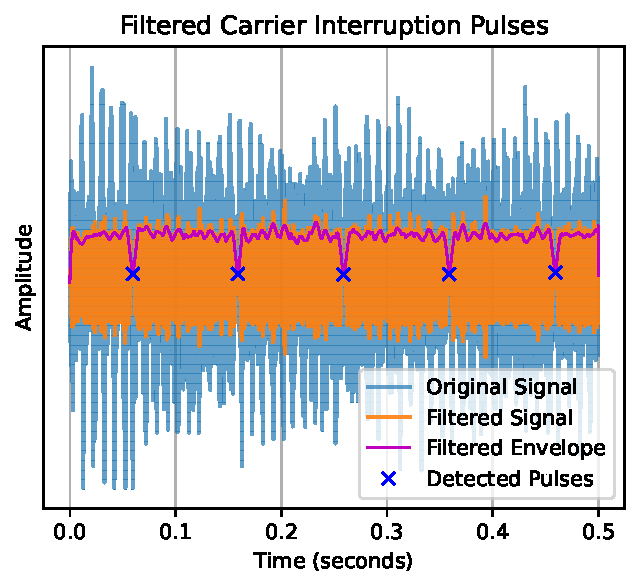
\includegraphics[height=0.8\textwidth]{carrier-filtered.pdf}
    \captionsetup{width=0.9\textwidth}
    \caption{Isolated 10 Hz interruptions}
    \label{fig:carrier-filtered}
  \end{subfigure}
  \hfill
  \begin{subfigure}[b]{0.48\textwidth}
    \centering
    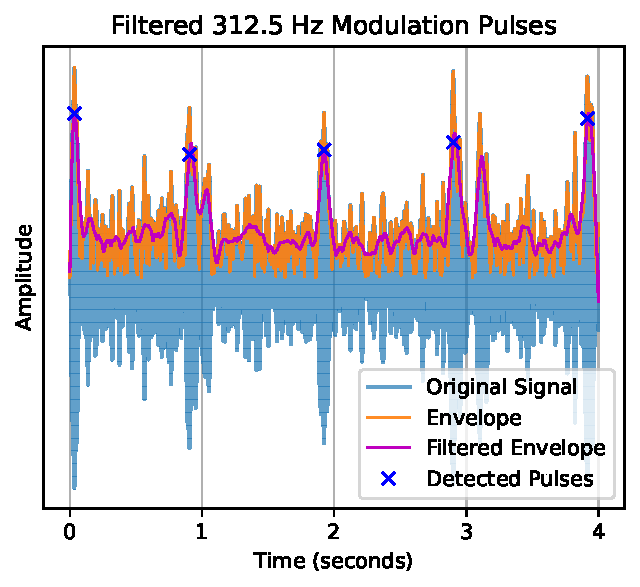
\includegraphics[height=0.8\textwidth]{312-filtered.pdf}
    \captionsetup{width=0.9\textwidth}
    \caption{Isolated 312.5 Hz modulations}
    \label{fig:312-filtered}
  \end{subfigure}
  \captionsetup{width=0.9\textwidth}
  \caption{Carrier signals filtered at target frequencies after DSP.}
  \label{fig:dsp-results}
\end{figure}

The results from the DSP stages are further visualized using a Matplotlib
library~\cite{pyplot} in Figure~\ref{fig:carrier-filtered} for the 10 Hz
carrier interruptions and Figure~\ref{fig:312-filtered} for the 312.5 Hz
modulations. Each figure displays the signal after the DSP and peak detection
steps have been applied, showcasing the target frequencies' signal
characteristics.

Following the isolation and detection of the 10 Hz carrier interruptions and
312.5 Hz modulations through digital signal processing (DSP) techniques, a
crucial step involves analyzing the peak timing information to compute the
phases of the target signals. This phase information is instrumental in
deriving precise time measurements from the RBU signal.

%To simplify handling of recurring signals this paper proposes utilization of
%modular arithmetic to consistently represent phases for all recurring signals.
%Phase of a recurring signal is measured as its found peaks times modulo signal's period.
%For example, a peak of 312.5~Hz signal modulation that occurred at 2542
%milliseconds since the start of the recording is though of as having a phase of
%42 milliseconds, computed as $542 \mod 1000$, as its period is 1 second. For
%10~Hz interrupts signal the modulus will bee 100 milliseconds.

To facilitate the consistent representation and analysis of recurring signals,
this paper advocates the use of modular arithmetic for phase calculations. The
phase of a recurring signal is determined by calculating the modulo of the peak
occurrence times relative to the signal’s period. For instance, a peak of the
312.5~Hz modulated signal occurring at 2542 milliseconds since the start of
the recording would be considered to have a phase of 542 milliseconds,
calculated as \(2542 \mod 1000\), because the period of this signal is 1
second. Similarly, for 10~Hz interruptions, which have a period of 100
milliseconds, the modulus of 100 milliseconds is used.

Modular representations simplify algorithmic accumulation and averaging of
recorded signals to achieve target phase detection accuracy.

\begin{figure}[H]
    \centering
    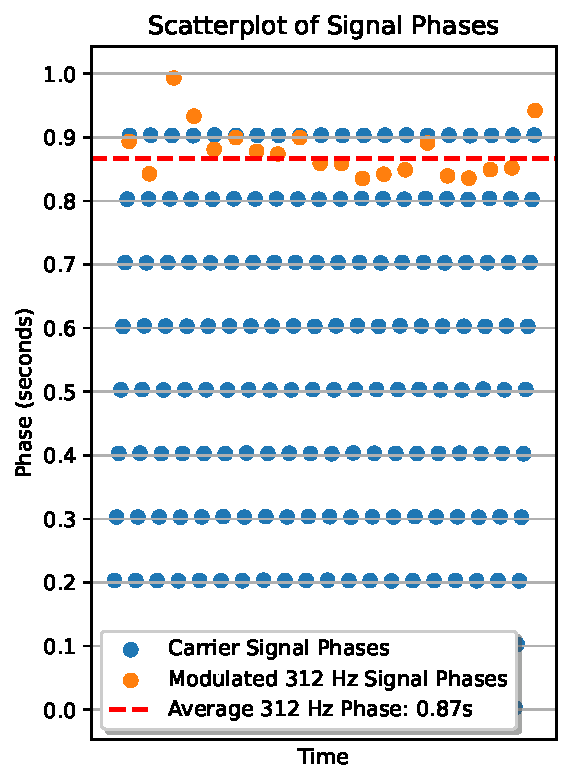
\includegraphics[width=0.45\textwidth]{signal-phases-scatter.pdf}
    \captionsetup{width=0.8\textwidth}
        \caption{Scatter plot displaying the phase values of detected signals
        peaks. The x-axis represents the time of peak occurrence since the
        recording began, and the y-axis shows the phase of each peak modulo 1
        second, highlighting the periodic nature of the peak occurrences.}
    \label{fig:signal-phases-scatter}
\end{figure}

Figure~\ref{fig:signal-phases-scatter} depicts the phases of all detected peaks
across two analyzed signals, corresponding to 1-second intervals. The
consistent and near-linear distribution of the carrier interruption peak phases
demonstrates the effectiveness of the DSP algorithms in accurately identifying
these markers. Notably, there are minimal deviations from the expected linear
trend, suggesting successful peak detection with negligible errors.

However, the peak phases of the 312.5 Hz modulation exhibit a slightly higher
degree of variability compared to the carrier interruption peaks due to it's
wider modulation time frame. While the majority of these peaks cluster around a
central value, there are a few outliers evident in the figure.

To mitigate the impact of these outliers and achieve a more robust phase
estimation for the 312.5 Hz modulation, averaging and outlier removal
techniques are employed.
By calculating the average phase value across a defined window of consecutive
peaks, outliers can be removed and phase recomputed with higher degree of precision.

\begin{figure}[H]
    \centering
    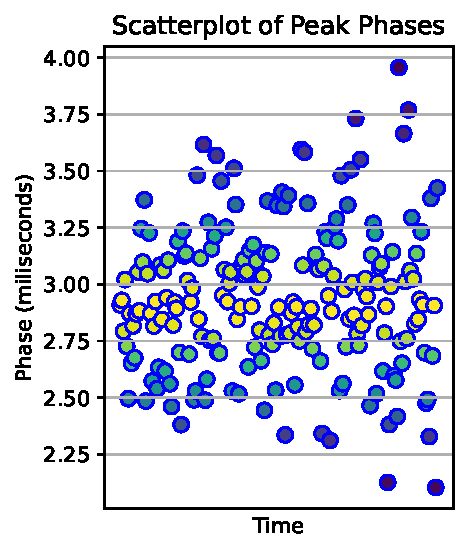
\includegraphics[width=0.4\textwidth]{carrier-phases-scatter.pdf}
    \captionsetup{width=0.8\textwidth}
    \caption{Phase values of carrier interruption peaks computed relative to
    it's period of 100 milliseconds with color representing phase-value
    density. }
    \label{fig:carrier-phases-scatter}
\end{figure}

Figure~\ref{fig:carrier-phases-scatter} presents a scatter plot depicting the
phases of individual carrier interruption peaks over a 30-second signal
duration (encompassing 300 detected peaks). This dataset
allows for a comprehensive evaluation and estimation of the phase error distribution.

Achieving a high degree of accuracy in time measurements is contingent upon the
precision with which phase values are extracted and analyzed. This paper
addresses the methodologies employed to evaluate and enhance the precision of
phase measurements derived from the RBU carrier interruptions.

To ensure the reliability of the time transfer technique, it is imperative to
ascertain that the phase measurements errors adhere to a predictable statistical
distribution. Initial analysis involves plotting the distribution of carrier
interruption phases to ascertain their conformity to a normal distribution,
which is a prerequisite for applying certain statistical techniques.

\begin{figure}[h]
    \centering
    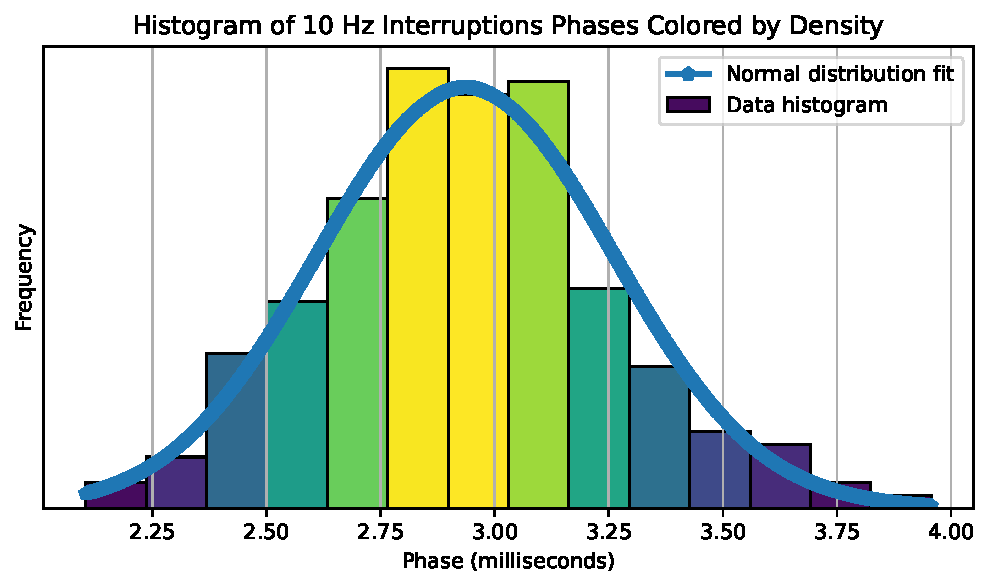
\includegraphics[width=0.7\textwidth]{carrier-phases-bins}
    \captionsetup{width=0.8\textwidth}
    \captionof{figure}{Distribution of carrier interruption phases,
        highlighting the Gaussian nature of the data.
        The x-axis represents the time of interruption occurrence since the
        recording began, and the y-axis shows the phase of each interruption
        modulo 100 milliseconds.
    }
    \label{fig:carrier-phases-bins}
\end{figure}

The histogram in Figure~\ref{fig:carrier-phases-bins} illustrates that the
phase values closely follow a normal distribution. This finding permits the
application of parametric statistical methods for further analysis.
Subsequently, the standard deviation (denoted as \(\sigma\)) of the phase
measurements is calculated, revealing a value of approximately 0.3
milliseconds. This measurement indicates the spread of the phase values around
the mean, serving as a metric of variability and precision.

In the context of refining measurement precision, it is essential to ascertain
the adequate number of samples needed to achieve a specified level of accuracy.
The desired precision, defined in terms of the standard error of the mean
(SEM), is set at 20 microseconds. This value is conservatively chosen based on
the consideration that light travels approximately 6 kilometers in this
duration, relating to less five percent of the operational range of typical
DVB-T2 systems, which extends up to 130 kilometers~\cite{lstelecom}. Furthermore,
the DVB-T2 provider has the option to reduce the target SEM by increasing the
sample size, which in turn affects the convergence speeds.

Using the standard deviation obtained from the
histogram analysis, the required sample size \(n\) is
calculated using the SEM equation:
\[
    \text{SEM} = \frac{\sigma}{\sqrt{n}};
\hspace{2em}
   n = \left(\frac{\sigma}{\text{SEM}}\right)^2
\]

Given \(\sigma = 0.3\) milliseconds and \(\text{SEM} = 0.02\) milliseconds, the
computation yields a sample size of approximately 289 measurements. This
calculation dictates the minimum number of phase measurements needed to achieve
the desired level of precision under normal distribution assumptions.

\pagebreak

\subsection{GNSS Jamming and Spoofing}

To anticipate and counteract potential threats in GNSS services, it is
imperative to simulate the actions of an attacker. This simulation uses readily
available tools to demonstrate potential vulnerabilities. A popular tool in
these simulations is the \textit{HackRF One} software-defined radio (SDR) from Great
Scott Gadgets.

The \texttt{osqzss/gps-sdr-sim} project is a prime example of an open-source
initiative that will be utilized in this study to conduct experimental spoofing
simulations. This software is highly cited and extensively employed within the
community for GNSS signal simulation, demonstrating its robustness and
reliability in such applications~\cite{gps-sdr-sim,spoofing1}.

\subsubsection{HackRF SDR Configuration}\label{sec:hackrf}

The maximum range for GNSS spoofing achieved with a HackRF One sans external
amplifiers is confined to roughly 5 meters, a finding documented by Songala et
al.~\cite{hackrf-gnss-spoofing}. This constraint is crucial for conducting
experiments within a safe and controlled environment. To further mitigate
risks, precautions were taken to comply with local regulation, execute the
experiments in secluded locations and restrict transmission durations, ensuring
minimal possibility of causing unintended disruptions.

Ephemeris data, which includes detailed information about the positions of
satellites in orbit, is crucial for generating accurate GNSS signals. This
data, typically provided in RINEXv3 format, is essential for ensuring that the
simulated signals reflect current satellite positions~\cite{rinex-v3}.

For the experiments, an antenna with a size of 10 cm was used. This dimension
corresponds to half the wavelength of the carrier frequency, calculated by the
equation:
\[
    \text{Wavelength} = \frac{c}{f} = \frac{3\times 10^8\ \text{m/s}}{1575 \times 10^{6}\ \text{Hz}}
    \approx 19\ \text{centimeters},
\]
where \( c \) is the speed of light and \( f \) is the frequency.

\begin{listing}[!ht]
\begin{minted}[tabsize=4, baselinestretch=1, breaklines=true, fontsize=\footnotesize]{bash}
./gps-sdr-sim -e ./ephemeris.rinex3 \  # Ephemeris data file
    -l "55.753,37.648,120" \ # Coordinates and height
    -b 8 \                   # 8-bit data format for HackRF DAC
    -o - |                   # Pipe output to standard output
    hackrf_transfer -t - \   # Read data from standard input
        -f 1575420000 \      # gnss carrier frequency of 1575.42MHz
        -s 2600000 \         # 2.6 Msps, maximum supported HackRF sample rate
\end{minted}
\caption{Command to simulate and transmit GNSS signal using HackRF.}
\label{lst:hackrf-tx}
\end{listing}

After setting up the HackRF with GPS-SDR-SIM and obtaining the latest ephemeris
data, signal simulation and transmission can commence as shown in
Listing~\ref{lst:hackrf-tx}.

Following successful signal transmission, the GNSS receiver typically converges
on the spoofed coordinates and time. This result is depicted in
Figure~\ref{fig:pygpsclient-spoofed}, showing a PyGPSClient interface reporting
the manipulated positioning.

\begin{figure}[h]
    \centering
    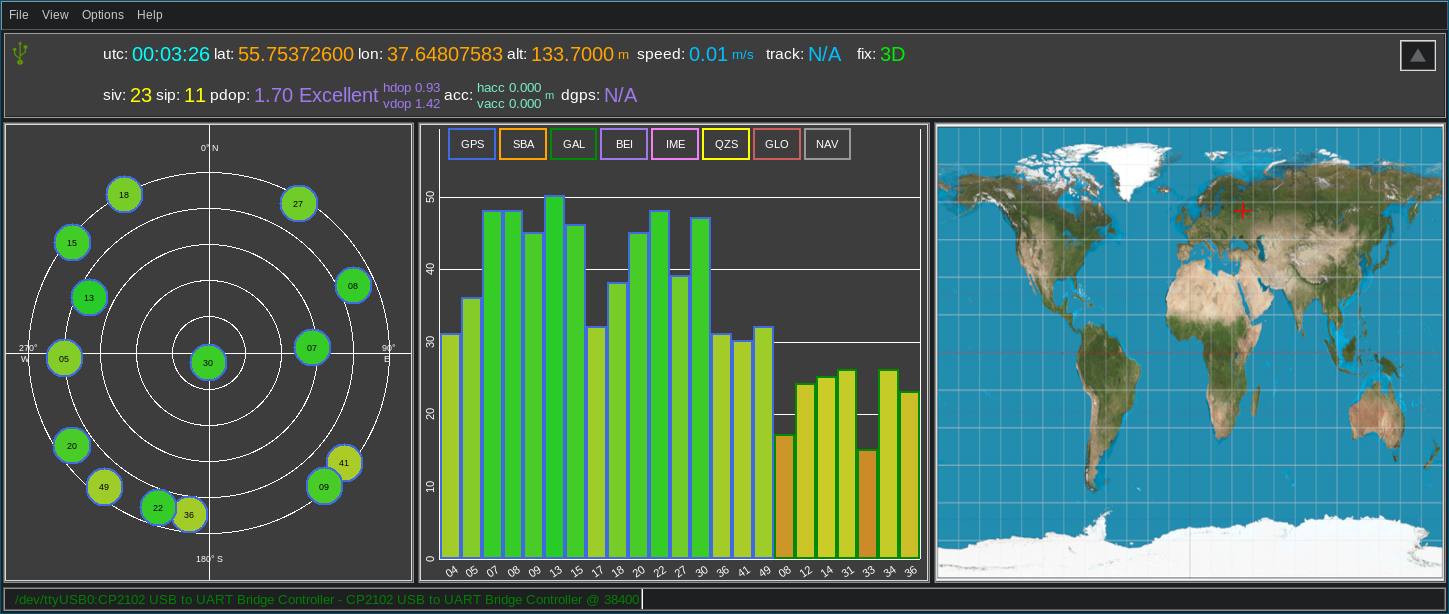
\includegraphics[width=0.7\textwidth]{pygpsclient-spoofed}
    \caption{PyGPSClient reporting spoofed position and time.}
    \label{fig:pygpsclient-spoofed}
\end{figure}


The proximity of the transmitter to the GNSS receiver results in exceptionally
high Carrier-to-Noise ratio ($C/N_0$) values, indicative of robust signal
reception. These values, depicted by green bins in the middle subplot of
Figure~\ref{fig:pygpsclient-spoofed}, suggest an unnaturally strong signal
relative to conventional GNSS reception levels. Elevated $C/N_0$ values can
serve as indicators of spoofing, offering a method for detection based on
signal strength anomalies~\cite{cn01,cn02}.

\begin{wrapfigure}{l}{0.50\textwidth}
    \centering
    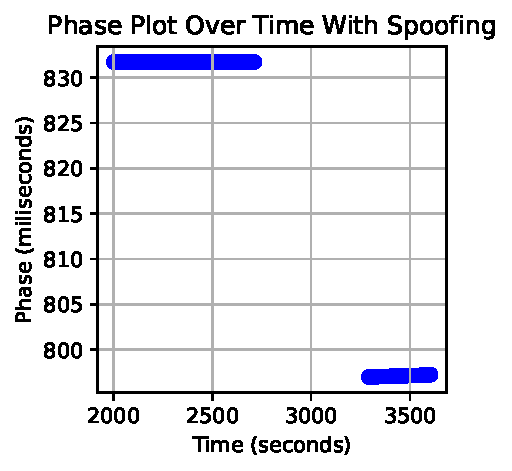
\includegraphics[width=0.48\textwidth]{phases-spoofed}
    \captionsetup{width=0.40\textwidth}
    \caption{Phase plot showing the effect of GNSS spoofing.}
    \label{fig:phases-spoofed}
\end{wrapfigure}


Additionally, plotting the phase of an incoming PPS signal as illustrated by
Figure~\ref{fig:phases-spoofed}, reveals a conspicuous change following the
activation of the HackRF transmission. The interruption in continuity between
the 2750 and 3250 second marks is attributable to the GNSS receiver's
reconvergence on the new, spoofed signal.

These observations not only underscore the efficacy and availability of the
spoofing technique but also highlight how discrepancies in $C/N_0$ and phase
continuity can be exploited to detect and mitigate spoofing attacks.

\subsection{Spoofing Detection Algorithm}

The work presented in this thesis proposes a comprehensive approach to
enhancing the resilience of GNSS time transfer by integrating longwave time
signals and standard-frequency radio stations as supplementary sources. This
hybrid method addresses vulnerabilities in GNSS, such as spoofing and signal
loss, by providing an independent verification mechanism through terrestrial
radio signals. The conclusion of this research not only encapsulates the
findings but also lays the groundwork for future innovations in the field of
time synchronization with alternative time sources.

The proposed method systematically leverages the stable and reliable nature of
longwave radio signals to augment GNSS time synchronization. The methodology
involves several key steps:
\begin{enumerate}[noitemsep]
    \item \textbf{Phase Establishment:} Initially, the correct relative phase
        of the radio time signal is compared to UTC time, established and
        stored. This phase acts as a benchmark for subsequent measurements.
    \item \textbf{Synchronization Delay:} While the GNSS receiver's
        pulse-per-second (PPS) provides primary time data, its synchronization
        is not immediately applied. Instead, synchronization values are
        computed and temporarily held.
    \item \textbf{Parallel Processing:} Concurrently, the radio time signal
        undergoes digital signal processing at a server to calculate time
        offsets accurately.
    \item \textbf{Validation and Application:} Time offsets are retransmitted
        to a time transfer device. Synchronization adjustments are only applied
        if the newly computed phase from the radio time station does not
        deviate beyond a predefined threshold from the stored phase.
    \item \textbf{Continuous Operation:} This process is iterative, ensuring
        ongoing verification and adjustment of time synchronization, thereby
        safeguarding against errors and potential spoofing attacks.
\end{enumerate}

\pagebreak
\section{Conclusions}\label{sec:concl}

%This research explores the integration of GNSS and longwave radio stations for
%enhancing time synchronization in SFN networks, addressing the vulnerabilities
%of GNSS systems. Through a multifaceted approach including literature review,
%analysis of GNSS vulnerabilities, exploration of alternative synchronization
%methods, and development of experimental devices, the study proposes a hybrid
%model for SFN synchronization. This approach not only aims to mitigate the
%risks associated with GNSS dependencies but also explores the potential of
%ground-based time signals for improving resilience and accuracy. The
%anticipated outcomes suggest promising directions for future research and
%practical applications in digital broadcasting networks, emphasizing the
%importance of diversifying time signal sources to ensure reliable and precise
%synchronization across SFN networks.

The significance of this research lies in its potential to provide another
decentralized time source and increase the reliability of time transfer systems
in critical infrastructure. By integrating a fail-safe mechanism that
cross-verifies GNSS data with longwave radio signals, the system maintains high
accuracy and robustness against disruptions. This method significantly
mitigates the risks associated with GNSS dependency, offering a more secure and
resilient framework for time-sensitive applications.

The experimental validations confirm the effectiveness of this approach, with
significant improvements in the reduction of time transmission errors and
enhanced resilience against disruptions. These findings lay a solid foundation
for future research and the development of advanced hybrid time synchronization
systems.

Looking forward, this thesis opens several avenues for further research:
\begin{itemize}[noitemsep]
    \item \textbf{Enhanced DSP Techniques:} Advanced digital signal processing
        algorithms can be explored to further reduce the time offset
        calculation latency and improve the precision of phase measurements.
    \item \textbf{Machine Learning Models:} Implementing machine learning
        techniques to predict and correct discrepancies in time signals before
        they affect the system could offer a proactive approach to time
        synchronization.
    \item \textbf{Broader Signal Integration:} Expanding the range of signal
        sources, including other radio frequencies and emerging satellite
        systems, could enhance the redundancy and reliability of the time
        transfer framework.
\end{itemize}

Finally, this thesis not only advances the academic field of time
synchronization but also provides a practical blueprint for deploying resilient
time transfer systems. The methodologies and insights derived from this study
contribute to the body of knowledge necessary for designing future-proof
synchronization systems that can operate reliably under adversarial conditions.

\pagebreak

\printbibliography[heading=bibintoc]

\pagebreak
\appendix

\section{Interrupt Handler Algorithm} \label{appendix:interrupt-algo}

\begin{minted}[linenos=true, tabsize=4, baselinestretch=1, breaklines=true, fontsize=\footnotesize]{rust}
#[embassy_executor::task]
async fn pps_sync_task(
    mut pps_exti_input: ExtiInput<'static>,
    mut pll_vcxo: DacChannel<'static, DAC1, 1, NoDma>,
) -> ! {
    let mut pll_dac_val: u16 = 2369;
    pll_vcxo.set(Value::Bit12Right(pll_dac_val));

    let mut count = 1;
    let mut sum = 0u64;
    const AVERAGING_COUNT: u64 = 100;
    let mut before = 0;

    loop {
        pps_exti_input.wait_for_rising_edge().await;
        let now = Instant::now().as_ticks();

        let diff = now - before;

        sum += diff;
        if count >= AVERAGING_COUNT {
            let avg = sum as f64 / AVERAGING_COUNT as f64;
            info!("Average diff: {}", avg);

            if sum > 10_000_000 * AVERAGING_COUNT {
                pll_dac_val -= 1;
            } else if sum < 10_000_000 * AVERAGING_COUNT {
                pll_dac_val += 1;
            }

            info!("Set DAC to: {}", pll_dac_val);
            pll_vcxo.set(Value::Bit12Right(pll_dac_val));

            sum = 0;
            count = 1;
        } else {
            count += 1;
            info!("PHASE: {}", now % 10_000_000);
        }

        before = now;
    }
}
\end{minted}

\end{document}
